\documentclass[9pt,mathserif,unknownkeysallowed]{beamer}
%\documentclass[9pt,mathserif,handout]{beamer}
\mode<presentation>
{
  \usetheme{Warsaw}
  \usecolortheme{crane}
  \setbeamercovered{transparent}
	\useoutertheme{split} 
	 
	\defbeamertemplate*{slidenumber}{framenumber} 
	     {\insertframenumber} 
	 \defbeamertemplate{slidenumber}{totalframenumber} 
	     {\insertframenumber\,/\,\inserttotalframenumber} 
	 \defbeamertemplate{slidenumber}{pagenumber} 
	     {\insertpagenumber} 
	 \defbeamertemplate{slidenumber}{totalpagenumber} 
	     {\insertpagenumber\,/\,\insertpresentationendpage} 
	 
	\defbeamertemplate*{footline}{split slidenumber right} 
	 {% 
	   \leavevmode% 
	   \hbox{\begin{beamercolorbox}
	[wd=.5\paperwidth,ht=2.5ex,dp=1.125ex,leftskip=.3cm plus1fill,rightskip=.3cm]
	{author in head/foot}% 
	     \usebeamerfont{author in head/foot}\insertshortauthor 
	   \end{beamercolorbox}% 
	   \begin{beamercolorbox}
	[wd=.5\paperwidth,ht=2.5ex,dp=1.125ex,leftskip=.3cm,rightskip=.3cm plus1fil]
	{title in head/foot}% 
	     \usebeamerfont{title in head/foot}\insertshorttitle% 
	     \hskip2ex plus1fill% 
	     \usebeamertemplate{slidenumber}% 
	   \end{beamercolorbox}}% 
	   \vskip0pt% 
	 
	} 
	 
	\defbeamertemplate{footline}{split slidenumber left} 
	 {% 
	   \leavevmode% 
	   \hbox{\begin{beamercolorbox}
	[wd=.5\paperwidth,ht=2.5ex,dp=1.125ex,leftskip=.3cm plus1fil,rightskip=.3cm]
	{author in head/foot}% 
	     \usebeamerfont{author in head/foot}% 
	     \usebeamertemplate{slidenumber}% 
	     \hskip2ex plus1fill% 
	     \insertshortauthor 
	   \end{beamercolorbox}% 
	   \begin{beamercolorbox}
	[wd=.5\paperwidth,ht=2.5ex,dp=1.125ex,leftskip=.3cm,rightskip=.3cm plus1fil]
	{title in head/foot}% 
	     \usebeamerfont{title in head/foot}\insertshorttitle% 
	   \end{beamercolorbox}}% 
	   \vskip0pt% 
	} 
}


\usepackage[english]{babel}
\usepackage[latin1]{inputenc}
\usepackage{times}
\usepackage[T1]{fontenc}
\usepackage{verbatim}

\usepackage{amsmath}
\usepackage{amssymb}
\usepackage{amsfonts}
\usepackage{pxfonts}
\usepackage{amsthm}
\usepackage{graphicx}
\usepackage{stmaryrd}


\usepackage{bussproofs}
\usepackage{proof}

\usepackage{fancybox}
\usepackage{fancyvrb}

\usepackage{xspace}
\usepackage{pgf,pgfarrows,pgfnodes}

% \usepackage{tikz}
% \usepackage{pgfgantt}
% \usepackage{chronology}


%\usepackage{rotating}

% Sequent Calculus Proof Settings
\EnableBpAbbreviations
\def\fCenter{\mbox{\ $\vdash$\ }}

\usepackage{calculi}

% Logical symbols
\newcommand{\imp}{\rightarrow}
\newcommand{\biimp}{\leftrightarrow}
\newcommand{\allq}{\forall}
\newcommand{\all}{\forall}
\newcommand{\exq}{\exists}
\newcommand{\ex}{\exists}
\newcommand{\seq}{\vdash}
\newcommand{\nec}{\Box} % necessarily
\newcommand{\pos}{\Diamond} % possibly


\newcommand{\ess}[2]{#1 \ \mathit{ess} \ #2}
\newcommand{\NE}{E}

\newcommand{\s}{\qquad}

\def\modal#1{\boldsymbol{#1}}
\def\mfalse{\modal\bot}
\def\mtrue{\modal\top}
\def\mnot{\modal\neg\,}
\def\mor{\,\modal\vee\,}
\def\mand{\,\modal\wedge\,}
\def\mimpl{\,\modal\supset\,}
\def\miff{\,\modal\Leftrightarrow\,}
\def\mball#1{\modal\Box_{#1}\,}
\def\mdexi#1{\modal\Diamond_{#1}\,}
\def\mall#1{\modal{\forall}{#1}\lambdot\,}
\def\mallprop#1{\modal{\forall^{p}}{#1}\lambdot\,}
\def\mallind#1{\modal{\forall^{\mu}}{#1}\lambdot\,}
\def\mexi#1{\modal{\exists}{#1}\lambdot\,}
\def\mpi{\modal{\Pi}\,}
\def\mvalid{\modal{\texttt{valid}}} 

\def\typearrow{\shortrightarrow}
\def\worldtype{\iota}
\def\indtype{\mu}


\def\lambdot{\rule{0.6mm}{0.6mm}\hspace{0.4ex}} 
\def\all#1{\forall #1\lambdot}
\def\exi#1{\exists #1\lambdot}
\def\lam#1{\lambda #1\lambdot}


\newcommand\entity[1]{\text{\textrm{#1}}}
\def\QHL{\entity{QHL}}
\def\QML{\entity{HOML}}
\def\NOM{\entity{NOM}}
\def\SVAR{\entity{SVAR}}
\def\CON{\entity{CON}}
\def\FVAR{\entity{FVAR}}
%\def\IC{\entity{IC}}
\def\FSYM{\entity{FSYM}}
\def\RSYM{\entity{RSYM}}
\def\QHLSTT{\entity{QHLSTT}}
\def\QMLSTT{\entity{QMLSTT}}
\def\IV{\entity{IV}}
\def\PV{\entity{PV}}
\def\SYM{\entity{SYM}}
\def\IVSTT{\entity{IVSTT}}
\def\PVSTT{\entity{PVSTT}}
\def\SYMSTT{\entity{SYMSTT}}
\def\SSTT{\entity{SSTT}}
\def\AR{\entity{AR}}
\def\STT{\entity{STT}\xspace}

\def\QKPIm{\entity{QK}\pi^-\xspace}
\def\QKPI{\entity{QK}\pi\xspace}
\def\QKPIp{\entity{QK}\pi^+\xspace}
\def\QSFPIm{\entity{QS5}\pi^-\xspace}
\def\QSFPI{\entity{QS5}\pi\xspace}
\def\QSFPIp{\entity{QS5}\pi^+\xspace}

\def\stt{\entity{STT}\xspace}
\def\tt{\entity{STT}}
\def\lm{\entity{MM}\xspace}
\def\ipl{\entity{IPL}\xspace}
\def\HOML{\entity{HOML}\xspace}
\def\HOL{\entity{HOL}\xspace}

\def\worldtype{\mu}
\def\indtype{\iota}
\def\mutype{\mu}
\def\boola{\omicron}
\def\boolb{\hat{\omicron}}

\def\ar{\shortrightarrow}

\newcommand\hol[1]{\boldsymbol{#1}}
\newcommand\lift[1]{\lceil #1 \rceil}
\newcommand\llift[1]{\dot{#1}}

\usepackage{xparse}

\NewDocumentCommand{\framecolorbox}{oommm}
 {% #1 = width (optional)
  % #2 = inner alignment (optional)
  % #3 = frame color
  % #4 = background color
  % #5 = text
  \IfValueTF{#1}
   {%
    \IfValueTF{#2}
     {\fcolorbox{#3}{#4}{\makebox[#1][#2]{#5}}}
     {\fcolorbox{#3}{#4}{\makebox[#1]{#5}}}%
   }
   {\fcolorbox{#3}{#4}{#5}}%
 }

\newenvironment{transitionframe}[2]
{
\begin{frame}{} \Large
\centering
\colorbox{#2}{\includegraphics[height=.6\textheight]{#1}}
\vfill
}
{

\end{frame}
}

\newenvironment{changemargin}[2]{% 
  \begin{list}{}{% 
    \setlength{\topsep}{0pt}% 
    \setlength{\leftmargin}{#1}% 
    \setlength{\rightmargin}{#2}% 
    \setlength{\listparindent}{\parindent}% 
    \setlength{\itemindent}{\parindent}% 
    \setlength{\parsep}{\parskip}% 
  }% 
\item[]
}{\end{list}} 


\setlength{\fboxsep}{3pt}%
\setlength{\fboxrule}{2pt}%


\title[Automating G�del's Ontological Proof of God's Existence]
{
Automating G�del's Ontological Proof of God's Existence with Higher-order Automated Theorem Provers
}

\author{\textbf{Christoph Benzm\"{u}ller}\thanks{
   Supported by DFG grant BE 2501/9-1} and \textbf{Bruno Woltzenlogel Paleo}}


\date[20.08.2013]{20th of August 2014 \\[1em] ECAI 2014}

\begin{document}

\begin{frame}
  \titlepage
%\colorbox{gray}{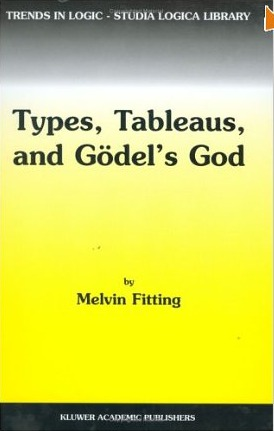
\includegraphics[height=2.5cm]{Images/Books/buch7.jpg} }
%\hfill
%\colorbox{gray}{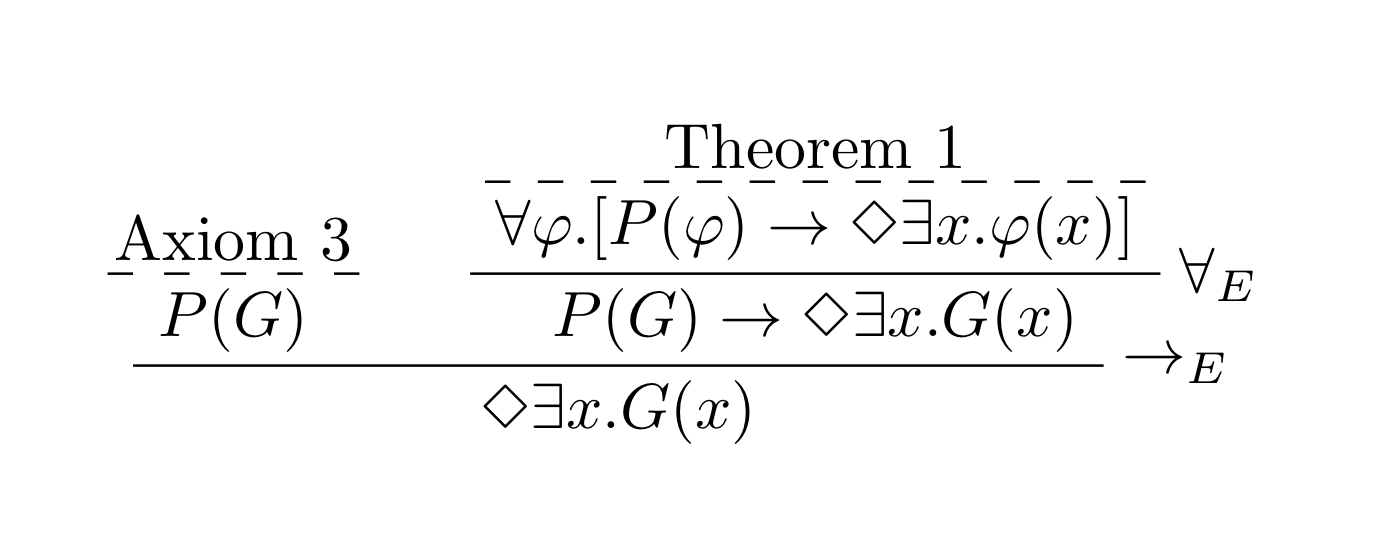
\includegraphics[height=2.5cm]{Images/ND.png}}
%\hfill \begin{footnotesize}A gift to \textbf{Priest Edvaldo} and his church in Piracicaba, Brazil\end{footnotesize}
\end{frame}

\begin{frame}{Vision of Leibniz (1646--1716): \textit{Calculemus!}}
\begin{changemargin}{-.5cm}{-.5cm}
\begin{minipage}{4cm}
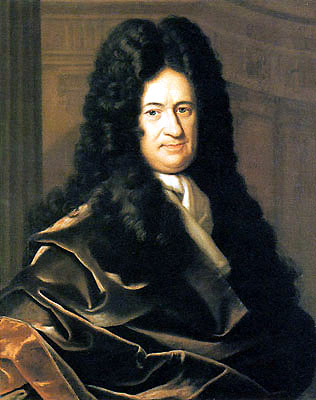
\includegraphics[width=4cm]{Images/Varia/Leibniz.png} 

\vspace*{1em}
\color{gray}\footnotesize
If controversies were to arise, there would be no more need of
disputation between two philosophers than between two
accountants. For it would suffice to take their pencils in their
hands, to sit down to their slates, and to say to each other \ldots :
Let us calculate. \\ \phantom{bla} \, \hfill (Translation by Russell)
\end{minipage} \hfill
\begin{minipage}{7cm} \small
Quo facto, quando orientur controversiae, non magis disputatione opus erit inter
duos philosophos, quam inter duos Computistas. Sufficiet enim calamos in
manus sumere sedereque ad abacos, et sibi mutuo \ldots dicere: calculemus.
\hfill (Leibniz, 1684)
\vspace*{1em}

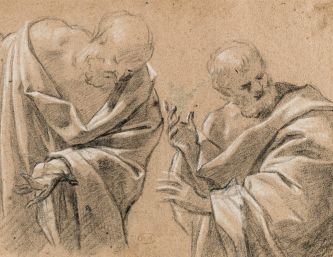
\includegraphics[width=7cm,height=5cm]{Images/Varia/Dispute1.jpg}

\vspace*{1em}
Required: \\
\, \hfil \textbf{characteristica universalis} and  \textbf{calculus ratiocinator}
\end{minipage}
\end{changemargin}
\end{frame}


\begin{frame}{Our Contribution: Towards a Computational Metaphysics}
\large
Ontological argument for the existence of God
\vfill
We focused on G�del's modern version in higher-order modal logic
\vfill
Automation with provers for higher-order classical logic (HOL)
\begin{itemize}
\item confirmation of known results
\item detection of some novel results
\item systematic variation of the logic settings
\item exploited HOL as a universal metalogic \\(characteristica universalis)
\end{itemize}
\end{frame}


\begin{frame}{A Long History}{\textcolor{blue}{pros} and \textcolor{red}{cons}} \Large
\begin{changemargin}{-.2cm}{0cm}
\hskip-.5em
\ldots\rotatebox[origin = bl,width = 0mm]{65}{\textcolor{blue}{Anselm v. C.}} \hskip-2.3em
          \rotatebox[origin = bl]{65}{\textcolor{red}{Gaunilo}} \hskip-1.3em
\ldots  \rotatebox[origin = bl]{65}{\textcolor{red}{Th. Aquinas}}  \hskip-2.3em
\ldots\ldots   \rotatebox[origin = bl]{65}{\textcolor{blue}{Descartes}} \hskip-1.7em
               \rotatebox[origin = bl]{65}{\textcolor{blue}{Spinoza}} \hskip-1.3em
               \rotatebox[origin = bl]{65}{\textcolor{blue}{Leibniz}}  \hskip-1.2em
\ldots  \rotatebox[origin = bl]{65}{\textcolor{red}{Hume}}  \hskip-1em
          \rotatebox[origin = bl]{65}{\textcolor{red}{Kant}}  \hskip-.8em
\ldots  \rotatebox[origin = bl]{65}{\textcolor{blue}{Hegel}}  \hskip-1.3em
\ldots  \rotatebox[origin = bl]{65}{\textcolor{red}{Frege}}  \hskip-1.3em
\ldots  \rotatebox[origin = bl]{65}{\textcolor{blue}{Hartshorne}} \hskip-1.9em
          \rotatebox[origin = bl]{65}{\textcolor{blue}{Malcolm}}  \hskip-1.4em
          \rotatebox[origin = bl]{65}{\textcolor{red}{Lewis}}  \hskip-1em
          \rotatebox[origin = bl]{65}{\textcolor{blue}{Plantinga}}  \hskip-1.6em
          \rotatebox[origin = bl]{65}{\textcolor{blue}{G\"odel}}   \hskip-1.2em
\ldots \\[1em]


\onslide<2->
{
\vfill
Anselm's notion of God (Proslogion, 1078):\\
\,\hfill \textbf{``God is that, than which nothing greater can be
  conceived.''} \\[1em]
}

\onslide<3->
{
G\"odel's notion of God:\\
\,\hfill \textbf{``A God-like being possesses all `positive'
  properties.''} \\[1em]
}

\onslide<2->
{
To show by logical reasoning: \\
\,\hfill \textbf{``\alt<3>{Necessarily God exists.}{God exists.}''} \\
\,\hfill \alt<3>{${\nec} \exq x G(x)$}{$\exq x G(x)$}\\[1em]
}
\end{changemargin}
\end{frame}



\begin{frame}{The Ontological Proof Today}
\vskip1em
% \emph{\huge Wohl eine jede Philosophie kreist um den ontologischen
%   Gottesbeweis} \\[1.5em]
% (Adorno, Negative Dialektik, 1966)
% \vfill
\begin{center}

\hfill
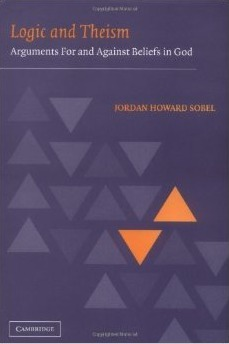
\includegraphics[height=2.2cm]{Images/Books/buch3.jpg} \hfill

\includegraphics[height=2.2cm]{Images/Books/buch2.jpg} \hfill 
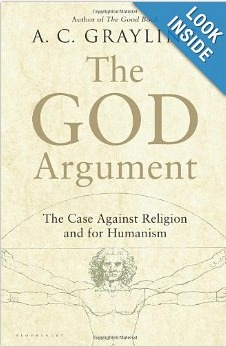
\includegraphics[height=2.2cm]{Images/Books/buch4.jpg} \hfill
\hfill

\vspace{0.5 cm}

\hfill
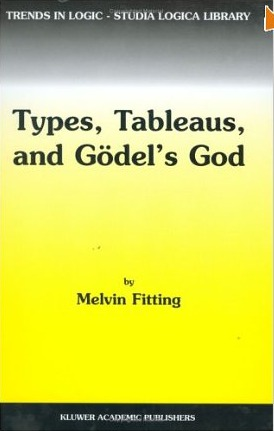
\includegraphics[height=2.2cm]{Images/Books/buch7.jpg} \hfill
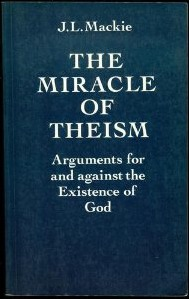
\includegraphics[height=2.2cm]{Images/Books/buch5.jpg} \hfill
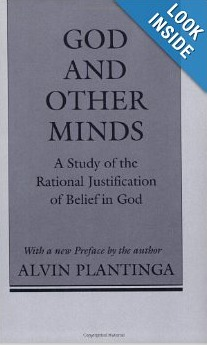
\includegraphics[height=2.2cm]{Images/Books/buch6.jpg} \hfill

\includegraphics[height=2.2cm]{Images/Books/buch1.jpg} \hfill
\hfill

\vspace{0.5 cm}

\hfill
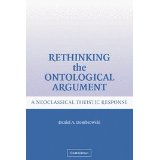
\includegraphics[height=2.2cm]{Images/Books/buch8.jpg} \hfill
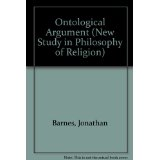
\includegraphics[height=2.2cm]{Images/Books/buch9.jpg} \hfill
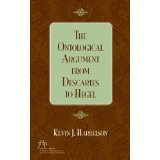
\includegraphics[height=2.2cm]{Images/Books/buch10.jpg} \hfill
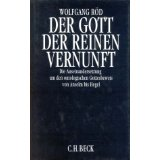
\includegraphics[height=2.2cm]{Images/Books/buch11.jpg} \hfill
\hfill

\end{center}
\end{frame}




\begin{frame}{G\"odel's Manuscript: 1930's, 1941, 1946-1955, 1970}
\bigskip

\begin{changemargin}{-1.2cm}{-1.2cm}
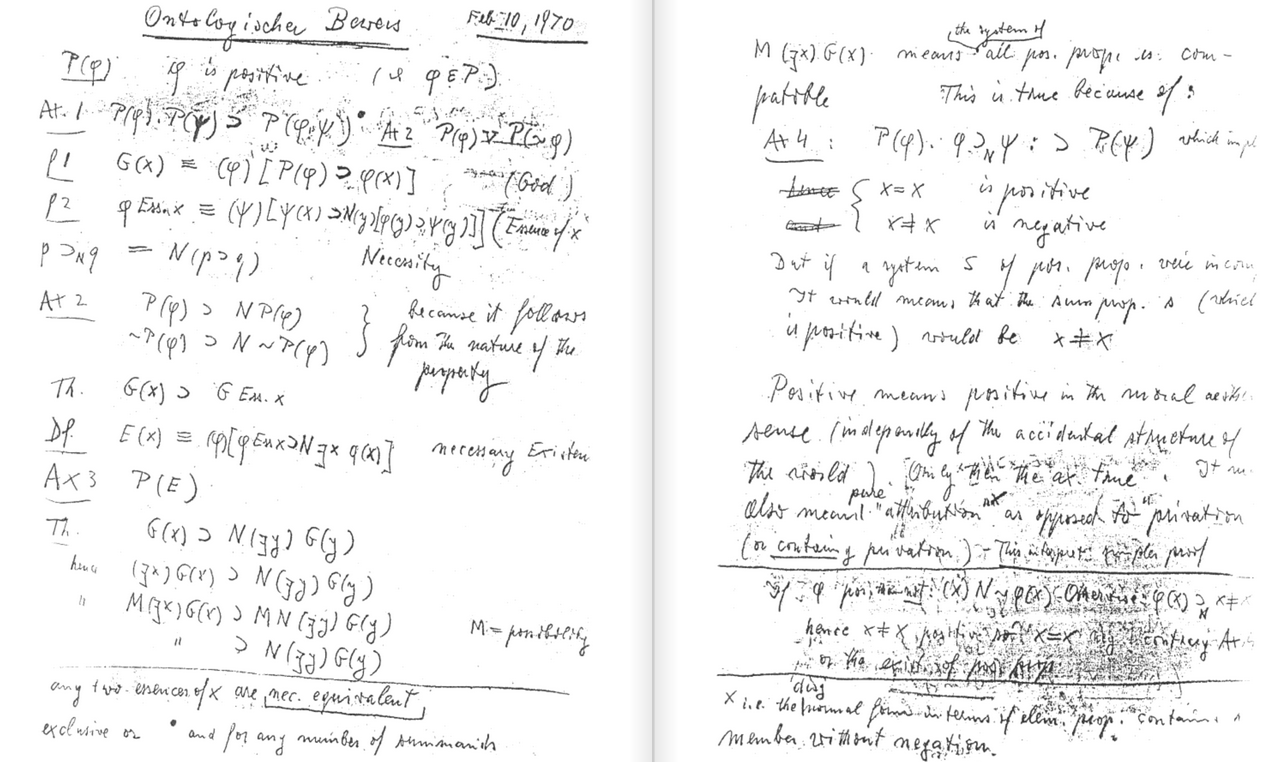
\includegraphics[width=13cm]{Images/Manuscript.png}
\end{changemargin}
\end{frame}




\def\scottproof{
\resizebox{\textwidth}{!}{
\begin{minipage}{12cm}%\small
\begin{itemize}
\item[Axiom A1] Either a property or its negation is positive, but not
  both: \hfill 
  ${\alt<3>{\textcolor{red}{\allq \phi}}{\allq \phi} [P(\neg \phi) \biimp \neg P(\phi)]}$ 
\item[Axiom A2] A property necessarily implied by a
  positive property is positive:  \phantom{bla bla bla bla bla bla bla}  \hfill 
  ${\alt<3>{\textcolor{red}{\allq \phi \allq \psi}}{\allq \phi \allq \psi} [(P(\phi) \wedge \alt<2>{\textcolor{red}{\nec}}{\nec} \allq x [\phi(x)
  \imp \psi(x)]) \imp P(\psi)]}$ 
\item[\textcolor{blue}{Thm. T1}] \textcolor{blue}{Positive properties are possibly exemplified:} \hfill \textcolor{blue}{${\alt<3>{\textcolor{red}{\allq \phi}}{\allq \phi} [P(\phi) \imp \alt<2>{\textcolor{red}{\pos}}{\pos}  \exq x \phi(x)]}$}
\item[Def. D1] A \emph{God-like} being possesses all positive properties: \hfill
  ${G(x) \biimp \alt<3>{\textcolor{red}{\allq \phi}}{\allq \phi} [P(\phi) \imp \phi(x)]}$ 
\item[Axiom A3]  The property of being God-like is positive: \hfill   ${P(G)}$ 
\item[\textcolor{blue}{Cor. C\phantom{1}}] \textcolor{blue}{Possibly, God exists:}\hfill \textcolor{blue}{${\alt<2>{\textcolor{red}{\pos}}{\pos} \exq x G(x)}$}
\item[Axiom A4]  Positive properties are necessarily positive: \hfill 
  ${\alt<3>{\textcolor{red}{\allq \phi}}{\allq \phi} [P(\phi) \imp \alt<2>{\textcolor{red}{\nec}}{\nec} P(\phi)]}$ 
\item[Def. D2] An \emph{essence} of an individual is a property possessed by it and necessarily implying any of its properties: \hfill ${\ess{\phi}{x} \biimp \alt<4>{\textcolor{red}{\phi(x)\,\wedge\,}}{\phi(x)\,\wedge\,}\alt<3>{\textcolor{red}{\allq \psi}}{\allq \psi} (\psi(x) \imp \alt<2>{\textcolor{red}{\nec}}{\nec} \allq y (\phi(y) \imp \psi(y)))}$ 
\item[\textcolor{blue}{Thm. T2}]  \textcolor{blue}{Being God-like is an essence of any
  God-like being:}  \hfill \textcolor{blue}{${\allq x [G(x) \imp \ess{G}{x}]}$}
\item[Def. D3] \emph{Necessary existence} of an individual~is the necessary exemplification of all its essences: 
  \phantom{b} \hfill ${\NE(x) \biimp \alt<3>{\textcolor{red}{\allq \phi}}{\allq \phi} [\ess{\phi}{x} \imp \alt<2>{\textcolor{red}{\nec}}{\nec}  \exq y \phi(y)]}$
\item[Axiom A5] Necessary existence is a positive property: \hfill ${P(\NE)}$ 
\item[\textcolor{blue}{Thm. T3}] \textcolor{blue}{Necessarily, God exists:} \hfill \textcolor{blue}{${\alt<2>{\textcolor{red}{\nec}}{\nec} \exq x G(x)}$}
\end{itemize}
\end{minipage}
}}


\def\scottproofsimple{
\resizebox{\textwidth}{!}{
\begin{minipage}{12cm}%\small
\begin{itemize}
\item[Axiom A1] Either a property or its negation is positive, but not
  both: \hfill 
  ${\alt<0>{\textcolor{red}{\allq \phi}}{\allq \phi} [P(\neg \phi) \biimp \neg P(\phi)]}$ 
\item[Axiom A2] A property necessarily implied by a
  positive property is positive:  \phantom{bla bla bla bla bla bla bla}  \hfill 
  ${\alt<0>{\textcolor{red}{\allq \phi \allq \psi}}{\allq \phi \allq \psi} [(P(\phi) \wedge \alt<0>{\textcolor{red}{\nec}}{\nec} \allq x [\phi(x)
  \imp \psi(x)]) \imp P(\psi)]}$ 
\item[\textcolor{blue}{Thm. T1}] \textcolor{blue}{Positive properties are possibly exemplified:} \hfill \textcolor{blue}{${\alt<0>{\textcolor{red}{\allq \phi}}{\allq \phi} [P(\phi) \imp \alt<0>{\textcolor{red}{\pos}}{\pos}  \exq x \phi(x)]}$}
\item[Def. D1] A \emph{God-like} being possesses all positive properties: \hfill
  ${G(x) \biimp \alt<0>{\textcolor{red}{\allq \phi}}{\allq \phi} [P(\phi) \imp \phi(x)]}$ 
\item[Axiom A3]  The property of being God-like is positive: \hfill   ${P(G)}$ 
\item[\textcolor{blue}{Cor. C\phantom{1}}] \textcolor{blue}{Possibly, God exists:}\hfill \textcolor{blue}{${\alt<0>{\textcolor{red}{\pos}}{\pos} \exq x G(x)}$}
\item[Axiom A4]  Positive properties are necessarily positive: \hfill 
  ${\alt<0>{\textcolor{red}{\allq \phi}}{\allq \phi} [P(\phi) \imp \alt<0>{\textcolor{red}{\nec}}{\nec} P(\phi)]}$ 
\item[Def. D2] An \emph{essence} of an individual is a property possessed by it and necessarily implying any of its properties: \hfill ${\ess{\phi}{x} \biimp \alt<0>{\textcolor{red}{\phi(x)\,\wedge\,}}{\phi(x)\,\wedge\,}\alt<0>{\textcolor{red}{\allq \psi}}{\allq \psi} (\psi(x) \imp \alt<0>{\textcolor{red}{\nec}}{\nec} \allq y (\phi(y) \imp \psi(y)))}$ 
\item[\textcolor{blue}{Thm. T2}]  \textcolor{blue}{Being God-like is an essence of any
  God-like being:}  \hfill \textcolor{blue}{${\allq x [G(x) \imp \ess{G}{x}]}$}
\item[Def. D3] \emph{Necessary existence} of an individual~is the necessary exemplification of all its essences: 
  \phantom{b} \hfill ${\NE(x) \biimp \alt<0>{\textcolor{red}{\allq \phi}}{\allq \phi} [\ess{\phi}{x} \imp \alt<0>{\textcolor{red}{\nec}}{\nec}  \exq y \phi(y)]}$
\item[Axiom A5] Necessary existence is a positive property: \hfill ${P(\NE)}$ 
\item[\textcolor{blue}{Thm. T3}] \textcolor{blue}{Necessarily, God exists:} \hfill \textcolor{blue}{${\alt<0>{\textcolor{red}{\nec}}{\nec} \exq x G(x)}$}
\end{itemize}
\end{minipage}
}}


\begin{frame}{Scott's Version of G\"odel's Axioms, Definitions and
    Theorems}
\begin{changemargin}{-.2cm}{-.5cm}
\begin{pgfpicture}{0cm}{0cm}{11cm}{11cm}
\pgfsetlinewidth{5\pgflinewidth} 
%\pgfsetendarrow{\pgfarrowto}
%\pgfsetstartarrow{\pgfarrowto}
%\pgfnodecircle{Node1}[stroke]{\pgfxy(0,9.5)}{0.25cm}
\pgfnodebox{Node0}[virtual]{\pgfxy(6,7.5)}{\begin{minipage}{11.5cm} \scottproofsimple\end{minipage}}{.2cm}{.2cm}
\end{pgfpicture}
\end{changemargin}
\end{frame}

\begin{frame}{Scott's Version of G\"odel's Axioms, Definitions and
    Theorems}
\begin{changemargin}{-.2cm}{-.5cm}
\begin{pgfpicture}{0cm}{0cm}{11cm}{11cm}
\pgfsetlinewidth{4\pgflinewidth} 
%\pgfsetendarrow{\pgfarrowto}
%\pgfsetstartarrow{\pgfarrowto}
%\pgfnodecircle{Node1}[stroke]{\pgfxy(0,9.5)}{0.25cm}
\pgfnodebox{Node0}[virtual]{\pgfxy(6,7.5)}{\begin{minipage}{11.5cm} \scottproofsimple\end{minipage}}{.2cm}{.2cm}
\pgfnodebox{Node1}[stroke]{\pgfxy(7.2,6.6)}{\phantom{B}}{.4cm}{.2cm}
\pgfnodebox{Node2}[virtual]{\pgfxy(7,3.5)}{
\framecolorbox[8.5cm][s]{blue}{blue!40}{
\begin{minipage}{8cm}\color{black} 
\vskip1em
\begin{center} Difference to G�del (who omits this conjunct) \end{center}
\phantom{bla}
\end{minipage}
}}{0pt}{0pt}
\pgfnodeconncurve{Node1}{Node2}{300}{120}{1cm}{1cm}
\end{pgfpicture}
\end{changemargin}
\end{frame}



\begin{frame}{Scott's Version of G\"odel's Axioms, Definitions and
    Theorems}
\begin{changemargin}{-.2cm}{-.5cm}
\begin{pgfpicture}{0cm}{0cm}{11cm}{11cm}
\pgfsetlinewidth{4\pgflinewidth} 
%\pgfsetendarrow{\pgfarrowto}
%\pgfsetstartarrow{\pgfarrowto}
%\pgfnodecircle{Node1}[stroke]{\pgfxy(0,9.5)}{0.25cm}
\pgfnodebox{Node0}[virtual]{\pgfxy(6,7.5)}{\begin{minipage}{11.5cm} \scottproofsimple\end{minipage}}{.2cm}{.2cm}
\pgfnodebox{Node1}[stroke]{\pgfxy(8.2,9.8)}{\phantom{B}}{.15cm}{.15cm}
\pgfnodebox{Node2}[stroke]{\pgfxy(10.6,7.9)}{\phantom{B}}{.15cm}{.15cm}
\pgfnodebox{NodeX}[virtual]{\pgfxy(7,3.5)}{
\framecolorbox[8.5cm][s]{blue}{blue!40}{
\begin{minipage}{8cm}\color{black} 
\vskip1em
\begin{center} Modal operators are used \end{center}
\phantom{bla}
\end{minipage}
}}{0pt}{0pt}
\pgfnodeconncurve{Node1}{NodeX}{270}{120}{1cm}{1cm}
\pgfnodeconncurve{Node2}{NodeX}{270}{110}{1cm}{1cm}
\end{pgfpicture}
\end{changemargin}
\end{frame}




\begin{frame}{Scott's Version of G\"odel's Axioms, Definitions and
    Theorems}
\begin{changemargin}{-.2cm}{-.5cm}
\begin{pgfpicture}{0cm}{0cm}{11cm}{11cm}
\pgfsetlinewidth{4\pgflinewidth} 
%\pgfsetendarrow{\pgfarrowto}
%\pgfsetstartarrow{\pgfarrowto}
%\pgfnodecircle{Node1}[stroke]{\pgfxy(0,9.5)}{0.25cm}
\pgfnodebox{Node0}[virtual]{\pgfxy(6,7.5)}{\begin{minipage}{11.5cm} \scottproofsimple\end{minipage}}{.2cm}{.2cm}
\pgfnodebox{Node1}[stroke]{\pgfxy(6.55,9.8)}{\phantom{B}}{.4cm}{.15cm}
\pgfnodebox{Node2}[stroke]{\pgfxy(9.65,8.8)}{\phantom{B}}{.15cm}{.15cm}
\pgfnodebox{NodeX}[virtual]{\pgfxy(7,3.5)}{
\framecolorbox[8.5cm][s]{blue}{blue!40}{
\begin{minipage}{8cm}\color{black} 
\vskip1em
\begin{center} second-order quantifiers \end{center}
\phantom{bla}
\end{minipage}
}}{0pt}{0pt}
\pgfnodeconncurve{Node1}{NodeX}{180}{120}{1cm}{1cm}
\pgfnodeconncurve{Node2}{NodeX}{270}{110}{1cm}{1cm}
\end{pgfpicture}
\end{changemargin}
\end{frame}




% \usebackgroundtemplate{}
% \begin{frame}{Scott's Version of G\"odel's Axioms, Definitions and Theorems}
% \scottproof
% \end{frame}



\begin{frame}[shrink]{Proof Overview}

$$
\textbf{D1: } G(x) \equiv \forall \varphi. [P(\varphi) \to \varphi(x)]
$$

$$
\textbf{D2: } \ess{\varphi}{x} \equiv \varphi(x) \wedge \all \psi. (\psi(x) \imp \nec \all x. (\varphi(x) \imp \psi(x)))
$$

$$
\textbf{D3: } NE(x) \equiv \all \varphi.[\ess{\varphi}{x} \imp \nec \ex y.\varphi(y)]
$$

\begin{prooftree}
\AXC{$\textbf{A3}$} \dashedLine
\UIC{$P(G)$}
		\AXC{$\textbf{A2}$} \dashedLine
		\UIC{$\all \varphi. \all \psi.[(P(\varphi) \wedge \nec \all x.[\varphi(x) \imp \psi(x)]) \imp P(\psi)]$}
					\AXC{$\textbf{A1a}$} \dashedLine
					\UIC{$\all \varphi. [P(\neg \varphi) \imp \neg P(\varphi)]$} \doubleLine
				\BIC{$\textbf{T1: } \all \varphi. [P(\varphi) \imp \pos \ex x.\varphi(x)]$} \doubleLine
	\BIC{$\textbf{C: } \pos \ex z. G(z)$}
\end{prooftree}





\begin{prooftree}
						\AXC{$\textbf{A1b}$} \dashedLine
						\UIC{$\all \varphi. [\neg P(\varphi) \imp P(\neg \varphi)]$}
								\AXC{$\textbf{A4}$} \dashedLine
								\UIC{$ \all \varphi.[P(\varphi) \to \Box \; P(\varphi)] $} \doubleLine
							\BIC{$\textbf{T2: } \all y.[G(y) \imp \ess{G}{y}]$}
									\AXC{$\textbf{A5}$} \dashedLine
									\UIC{$ P(NE) $} \doubleLine
								\BIC{$\textbf{L1: } \ex z. G(z) \imp \nec \ex x. G(x)$} \doubleLine
								\UIC{$\pos \ex z. G(z) \imp \pos \nec \ex x. G(x)$}
										\AXC{$\textbf{S5}$} \dashedLine
 										\UIC{$ \all \xi.[\pos \nec \xi \imp \nec \xi]$} \doubleLine	
									\BIC{$\textbf{L2: } \pos \ex z. G(z) \imp \nec \ex x. G(x)$}
\end{prooftree}

\begin{prooftree}
\AXC{$\textbf{C: } \pos \ex z. G(z)$}
		\AXC{$\textbf{L2: } \pos \ex z. G(z) \imp \nec \ex x. G(x)$} \doubleLine
	\BIC{$\textbf{T3: } \nec \ex x. G(x) $}
\end{prooftree}

\end{frame}


\begin{transitionframe}{Images/Transitions/GodComputerC}{black}
  \centering
\textbf{How to automate Higher-Order Modal Logic?}
%\\ into Higher-Order Logic}
%\textbf{Embedding Higher-Order Modal Logic \\ into Higher-Order Logic}
\end{transitionframe}

\begin{frame}{Embedding HOML in HOL} \large

  \hskip-1em Challenge: \hfill No provers for \emph{Higher-order Modal
    Logic\/} (\textcolor{red}{HOML}) \\[1em]

\hskip-1em Our solution: \hfill \textbf{Embedding in \emph{Higher-order Classical
  Logic\/} (\textcolor{blue}{HOL})} \\
\, \hfill Then use existing \textcolor{blue}{HOL} theorem provers for reasoning in \textcolor{red}{HOML} \\
\,\hfill {\small [Benzm\"ullerPaulson, Logica Universalis, 2013]}
\\[2em]

\hskip-1em Previous empirical findings:  \\[.5em]
\,\hfill Embedding of  \emph{First-order Modal Logic} in HOL works well 

\,\hfill {\small [Benzm\"ullerOttenRaths, ECAI, 2012]} \\
\,\hfill {\small [Benzm\"uller, LPAR, 2013]}
\end{frame}



\begin{frame}{Embedding HOML in HOL} \large
\begin{changemargin}{-.5cm}{0cm}

\textcolor{red}{HOML} \hfill
$\begin{array}{lll}\textcolor{red}{\varphi,\psi} & ::= &
  \textcolor{red}{\ldots}  \mid \textcolor{red}{\neg
    \varphi} \mid \textcolor{red}{\varphi \wedge \psi} \mid
  \textcolor{red}{\varphi \imp \psi}  \mid \textcolor{red}{\Box
    \varphi} \mid \textcolor{red}{\Diamond \varphi}  \mid
  \textcolor{red}{\forall {x}\, \varphi} \mid
  \textcolor{red}{\exists {x}\, \varphi} 
\mid \textcolor{red}{\forall {P}\, \varphi} \end{array}$ \\[1em]


\begin{itemize}
\item Kripke style semantics (possible world semantics)\\[2em]
\end{itemize}



\textcolor{blue}{HOL}\hfill 
$\begin{array}{lll}
\textcolor{blue}{s,t} & ::= & \textcolor{blue}{C}  \mid
\textcolor{blue}{x \mid \lambda{x} s} \mid \textcolor{blue}{s\, t}
\mid \textcolor{blue}{\neg s} \mid \textcolor{blue}{s \vee t} \mid
\textcolor{blue}{\forall {x}\, t} 
\end{array}$ \\[1em]

\begin{itemize}
\item Church's simple type theory \hfill {\small [Church, 1940],
    [Henkin, 1950]} \\[.5em]
\item various theorem provers exist \\[.5em]
  \quad interactive: \hfill Isabelle/HOL, HOL4, Hol Light, Coq/HOL, PVS,
  \ldots \\[.5em]
  \quad automated: \hfill TPS, LEO-II, Satallax, Nitpick, Isabelle/HOL, \ldots \\
\end{itemize}

\end{changemargin}
\end{frame}


\begin{frame}{Embedding HOML in HOL}\large
\begin{changemargin}{-.5cm}{0cm}

\textcolor{red}{HOML} \hfill
$\begin{array}{lll}\textcolor{red}{\varphi,\psi} & ::= &
  \textcolor{red}{\ldots}  \mid \textcolor{red}{\neg
    \varphi} \mid \textcolor{red}{\varphi \wedge \psi} \mid
  \textcolor{red}{\varphi \imp \psi}  \mid \textcolor{red}{\Box
    \varphi} \mid \textcolor{red}{\Diamond \varphi}  \mid
  \textcolor{red}{\forall {x}\, \varphi} \mid
  \textcolor{red}{\exists {x}\, \varphi} 
\mid \textcolor{red}{\forall {P}\, \varphi} \end{array}$ \\[1em]
\textcolor{blue}{HOL}\hfill 
$\begin{array}{lll}
\textcolor{blue}{s,t} & ::= & \textcolor{blue}{C}  \mid
\textcolor{blue}{x \mid \lambda{x} s} \mid \textcolor{blue}{s\, t}
\mid \textcolor{blue}{\neg s} \mid \textcolor{blue}{s \vee t} \mid
\textcolor{blue}{\forall {x}\, t} 
\end{array}$ \\[1em]

\pause

\textcolor{red}{HOML} in \textcolor{blue}{HOL}: \quad \textcolor{red}{HOML}
formulas $\textcolor{red}{\varphi}$ are mapped to
\textcolor{blue}{HOL} predicates $\textcolor{red}{\varphi_{\worldtype\typearrow o}}$

\begin{center}
\fcolorbox{blue}{white}{
$\begin{array}{lcl} 
    \textcolor{red}{\mnot} & = & \textcolor{blue}{
      \lambda{\varphi_{\worldtype\typearrow o}}\lambda{w_\worldtype}\neg \varphi w} \\ 
    \textcolor{red}{\mand} & = & \textcolor{blue}{ 
      \lambda{\varphi_{\worldtype\typearrow o}}
      \lambda{\psi_{\worldtype\typearrow o}} \lambda{w_\worldtype}
      (\varphi w \wedge \psi w)} \\ 
    \textcolor{red}{\imp} & = & \textcolor{blue}{ 
      \lambda{\varphi_{\worldtype\typearrow o}}
      \lambda{\psi_{\worldtype\typearrow o}} \lambda{w_\worldtype}
      (\neg \varphi w \vee \psi w)} \\ 
    \textcolor{red}{\forall} & = & \textcolor{blue}{ 
      \lambda{h_{\gamma\typearrow(\worldtype \typearrow o)}}
      \lambda{w_\worldtype} \forall {d_\gamma} \, h d w} \\
    \textcolor{red}{\exists} & = & \textcolor{blue}{ 
      \lambda{h_{\gamma\typearrow(\worldtype \typearrow o)}}
      \lambda{w_\worldtype} \exists {d_\gamma} \, h d w} \\
    \\
    \textcolor{red}{\Box} & = & \textcolor{blue}{ 
      \lambda{\varphi_{\worldtype\typearrow o}} \lambda{w_\worldtype}
      \forall {u_\worldtype}\, (\neg r w u \vee
      \varphi u)} \\ 
    \textcolor{red}{\Diamond} & = & \textcolor{blue}{ 
      \lambda{\varphi_{\worldtype\typearrow o}} \lambda{w_\worldtype}
      \exists {u_\worldtype}\, (r w u \wedge
      \varphi u)} \\ 
    \\
    \text{\textcolor{brown}{valid}} & = & \textcolor{blue}{
        \lambda{\varphi_{\worldtype\typearrow o}} \all{w_\worldtype}
        \varphi w}
\end{array}$
}  \quad \textcolor{blue}{Ax} 
\vskip1em
\end{center}

\pause

\quad The equations in \textcolor{blue}{Ax} are given as axioms to the \textcolor{blue}{HOL} provers! \\

\end{changemargin}
\end{frame}



\begin{frame}{Embedding HOML in HOL} \large

\hskip-1em Example \\[.5em]

 \textcolor{red}{HOML} formula  \hfill \textcolor{red}{$\Diamond \exists x G(x)$}

\pause 

 \textcolor{red}{HOML} formula in \textcolor{blue}{HOL}  \hfill $\text{\textcolor{brown}{valid}}\, \textcolor{red}{(\Diamond \exists x G(x))_{\worldtype\typearrow o}}$

\pause

expansion, $\beta\eta$-conversion \hfill $\textcolor{blue}{\forall
  w_\worldtype\textcolor{red}{(\Diamond \exists x
    G(x))_{\worldtype\typearrow o}}\, w}$ 

\pause

expansion, $\beta\eta$-conversion \hfill $\textcolor{blue}{\forall
  w_\worldtype \exists {u_\worldtype} (r w u \wedge
      \textcolor{red}{(\exists x G(x))_{\worldtype\typearrow o}} u)}$ 

% expansion, $\beta\eta$-conversion \hfill $\textcolor{blue}{\forall
%   w_\worldtype \exists {u_\worldtype} (r w u \wedge
%       \exists x \textcolor{red}{G(x)_{\worldtype\typearrow o}} u)}$ 

\pause

expansion, $\beta\eta$-conversion \hfill $\textcolor{blue}{\forall
  w_\worldtype \exists {u_\worldtype} (r w u \wedge
      \exists x G x u)}$ \\[1em]

\pause
\hskip-1em Expansion: \hfill user or prover may flexibly choose
expansion depth 

\pause
\vfill
\begin{block}{What are we doing?}
\vskip.5em
In order to prove that $\textcolor{red}{\varphi}$ is valid in \textcolor{red}{HOML}, \\
--> we instead prove that 
$\text{\textcolor{brown}{valid}}\,
\textcolor{red}{\varphi_{\worldtype\typearrow o}}$ can be derived
from \textcolor{blue}{Ax} in \textcolor{blue}{HOL}. \\[1em]

This can be done with interactive or automated \textcolor{blue}{HOL} theorem provers.
\end{block}
\pause
\vfill
\pause
\hskip-1em For the experts: \hfill soundness and completeness wrt Henkin semantics

\end{frame}


% \begin{transitionframe}{Images/Transitions/GodComputerC}{black}
% \textbf{
% \quad Automated Proof Search and Consistency Check \hfill  \\
% }
% \end{transitionframe}


\begin{frame}{Automated Theorem Provers and Model Finders for HOL}
\includegraphics[width=1.05\textwidth]{Images/HOLProversGrab}
\end{frame}


\begin{frame}{Proof Automation and Consistency Checking with \textsc{HOL-P}} \large
\colorbox{gray}{\includegraphics[width=\textwidth]{Images/Demos/DemoGrap}} 
\vfill 
Provers are called remotely in Miami --- no local installation needed!
\vfill
Download our experiments from \url{https://github.com/FormalTheology/GoedelGod/tree/master/Formalizations/THF}
\end{frame}

\begin{frame}{Interaction and Automation in Proof Assistant \textsc{Isabelle/HOL}} \large \centering
\colorbox{gray}{\includegraphics[width=.8\textwidth]{Images/Demos/IsabelleDemoGrab}}\vfill
See verifiable Isabelle/HOL journal article at: \url{http://afp.sourceforge.net/entries/GoedelGod.shtml}
\end{frame}

\begin{frame}{Interaction in Proof Assistant \textsc{Coq}} \large \centering
\colorbox{gray}{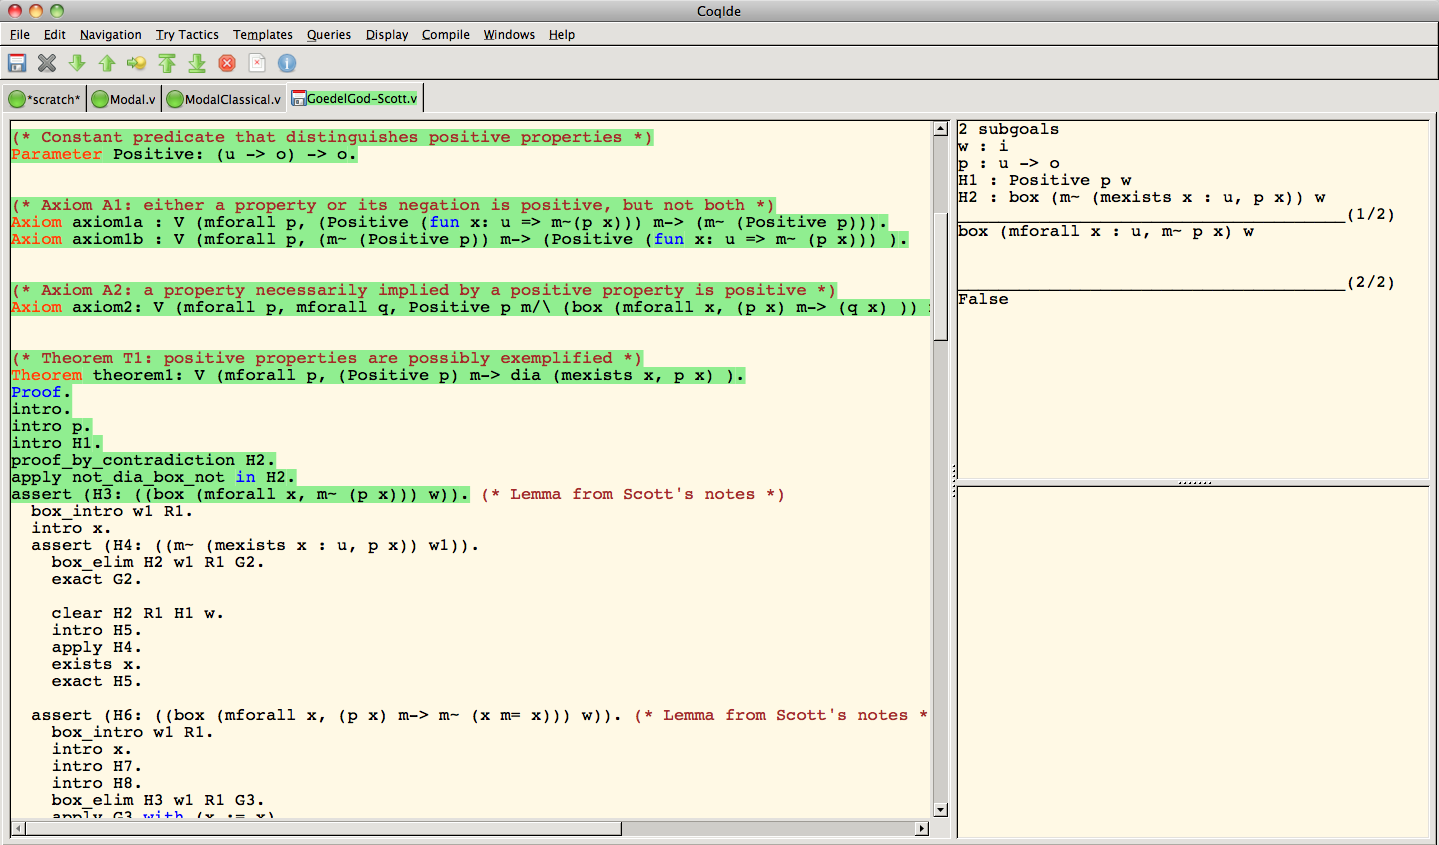
\includegraphics[width=1\textwidth]{Images/Demos/CoqDemo.png}}
\vfill
See verifiable Coq document at: \url{https://github.com/FormalTheology/GoedelGod/tree/master/Formalizations/Coq}
\end{frame}

% \begin{frame}{Results}
% \begin{changemargin}{-0.8cm}{-1.1cm}
% 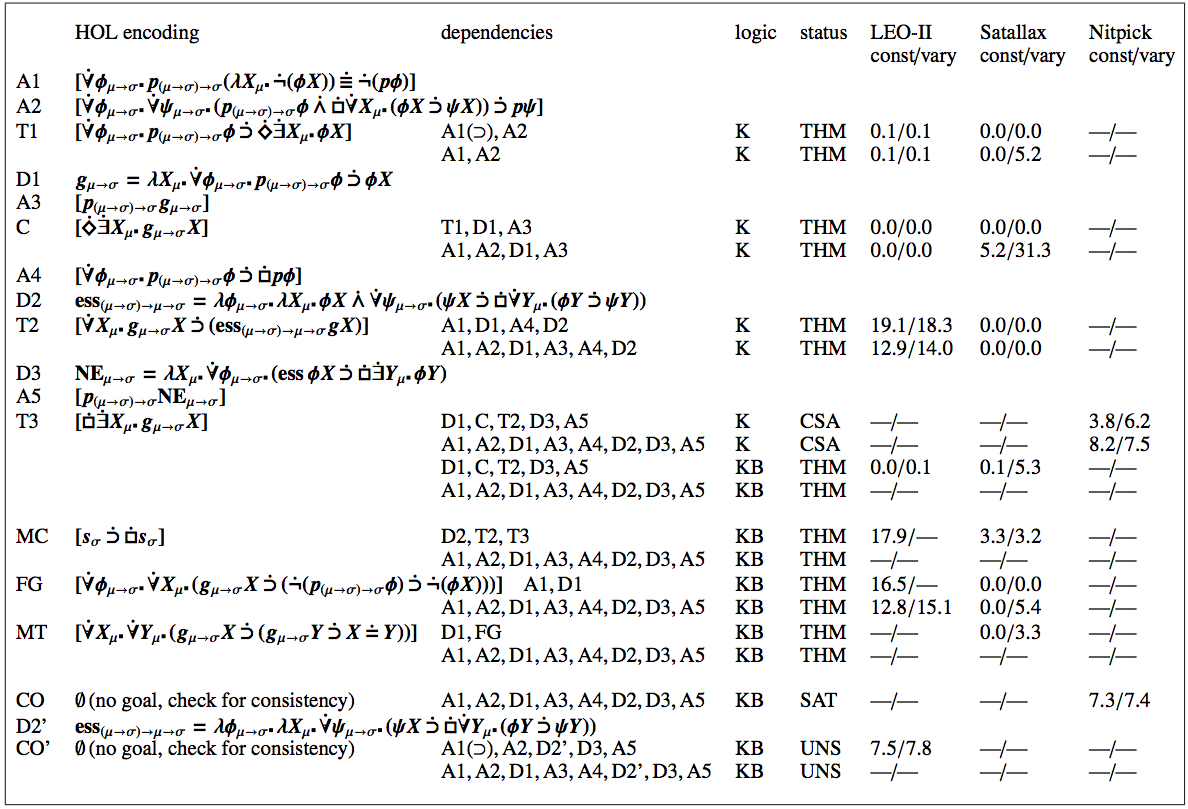
\includegraphics[width=12.4cm]{Images/Results.png}
% \end{changemargin}
% \end{frame}


\begin{transitionframe}{Images/Transitions/NietzscheGod3}{black}
\textbf{Main Findings}
\end{transitionframe}


\usebackgroundtemplate{
  \vbox to \paperheight{\vfil\hbox to \paperwidth{\hfil
      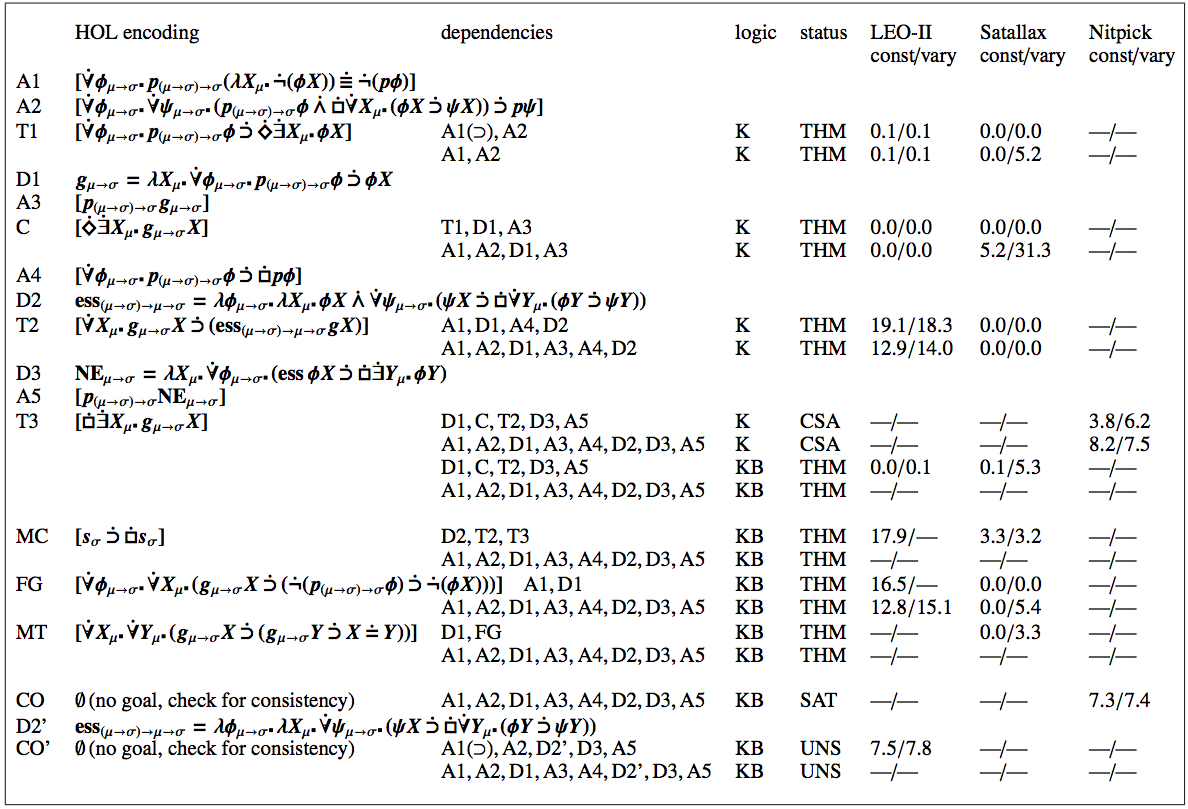
\includegraphics[width=11.5cm]{Images/Results.png} 
      \hfil}\vfil}
}
%\usebackgroundtemplate{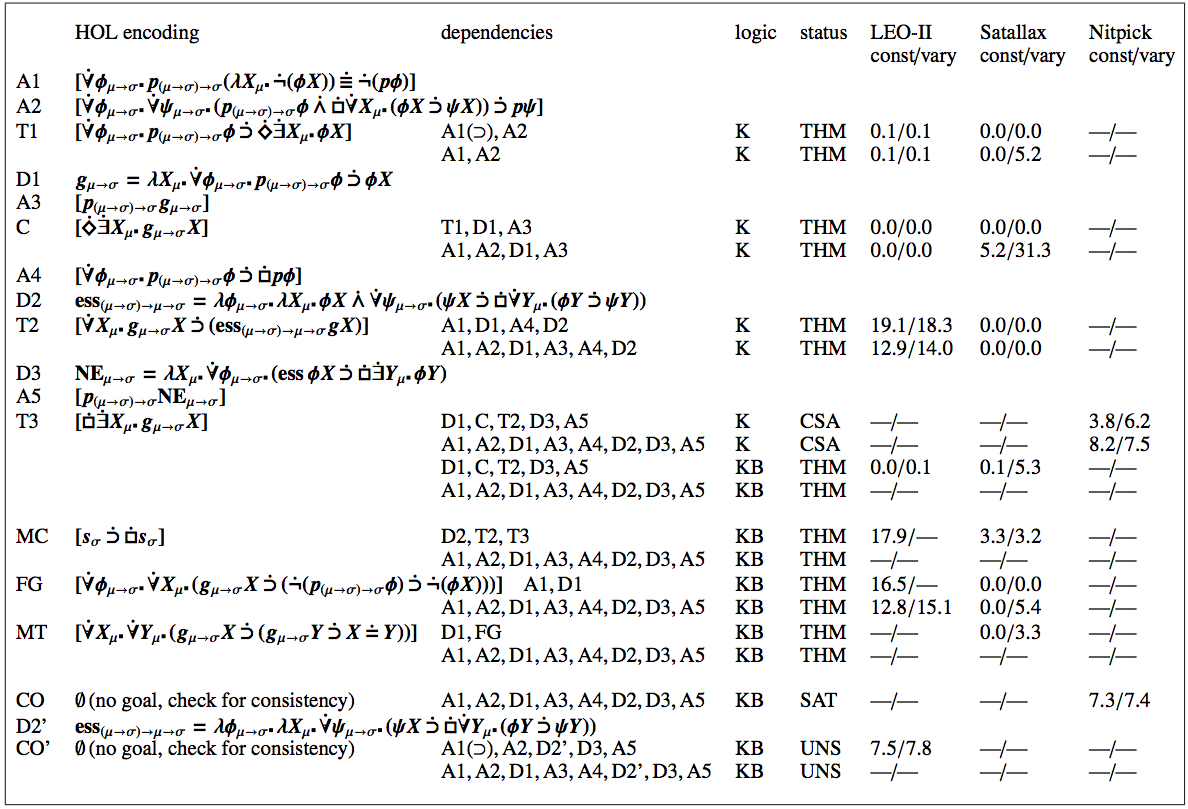
\includegraphics[width=\paperwidth]{Images/Results.png}}
%\pgfsetlinewidth{10\pgflinewidth} 
%\pgfsetlinecolor{blue} 

\begin{frame}{Main Findings}

\end{frame}

\begin{frame}{Main Findings}
\begin{changemargin}{-.2cm}{-.5cm}
\begin{pgfpicture}{0cm}{0cm}{11cm}{11cm}
\pgfsetlinewidth{5\pgflinewidth} 
\pgfsetendarrow{\pgfarrowto}
%\pgfsetstartarrow{\pgfarrowto}
%\pgfnodecircle{Node1}[stroke]{\pgfxy(0,9.5)}{0.25cm}
\pgfnodebox{Node1}[stroke]{\pgfxy(5.6,8)}{\phantom{Bla}}{5.6cm}{2.1cm}
\end{pgfpicture}
\end{changemargin}
\end{frame}

\setbeamercovered{invisible}

\begin{frame}{Main Findings}
\begin{changemargin}{-.2cm}{-.5cm}
\begin{pgfpicture}{0cm}{0cm}{11cm}{11cm}
\pgfsetlinewidth{5\pgflinewidth} 
\pgfsetendarrow{\pgfarrowto}
%\pgfsetstartarrow{\pgfarrowto}
%\pgfnodecircle{Node1}[stroke]{\pgfxy(0,9.5)}{0.25cm}
\pgfnodebox{Node1}[stroke]{\pgfxy(5.6,9.45)}{\phantom{Bla}}{5.6cm}{.2cm}
\pgfnodebox{Node2}[virtual]{\pgfxy(7,5)}{
\framecolorbox[8.5cm][s]{blue}{blue!40}{
\begin{minipage}{8cm}\color{black} \bf
%\vskip1em
\underline{Automating Scott's proof script} \\[1em]
{T1: "Positive properties are possibly exemplified"}
proved by LEO-II and Satallax 
\begin{itemize}
\item  in logic: K 
\item  from axioms:
  \begin{itemize} 
  \item A1 and A2
  \item \onslide<2->{\color{blue} A1($\supset$) and A2}
  \end{itemize}
\item for domain conditions: 
  \begin{itemize} 
  \item constant domains
  \item \onslide<3>{\color{blue} varying domains (individuals)}
  \end{itemize}
\end{itemize}
\vspace*{1em}
\end{minipage}
}}{2pt}{2pt}
\pgfnodeconncurve{Node1}{Node2}{180}{180}{1cm}{2cm}
\end{pgfpicture}
\end{changemargin}
\end{frame}

\begin{frame}{Main Findings}
\begin{changemargin}{-.2cm}{-.5cm}
\begin{pgfpicture}{0cm}{0cm}{11cm}{11cm}
\pgfsetlinewidth{5\pgflinewidth} 
\pgfsetendarrow{\pgfarrowto}
%\pgfsetstartarrow{\pgfarrowto}
%\pgfnodecircle{Node1}[stroke]{\pgfxy(0,9.5)}{0.25cm}
\pgfnodebox{Node1}[stroke]{\pgfxy(5.6,8.5)}{\phantom{Bla}}{5.6cm}{.2cm}
\pgfnodebox{Node2}[virtual]{\pgfxy(7,5)}{
\framecolorbox[8.5cm][s]{blue}{blue!40}{
\begin{minipage}{8cm}\color{black} \bf
%\vskip1em
\underline{Automating Scott's proof script} \\[1em]
C: "Possibly, God exists'' \\
proved by LEO-II and Satallax 
\begin{itemize}
\item  in logic: K 
\item  from assumptions:
  \begin{itemize} 
  \item T1, D1, A3
  \item A1, A2, D1, A3
  \end{itemize}
\item for domain conditions: 
  \begin{itemize} 
  \item constant domains
  \item varying domains (individuals)
  \end{itemize}
\end{itemize}
\vspace*{1em}
\end{minipage}
}}{2pt}{2pt}
\pgfnodeconncurve{Node1}{Node2}{180}{180}{1cm}{2cm}
\end{pgfpicture}
\end{changemargin}
\end{frame}


\begin{frame}{Main Findings}
\begin{changemargin}{-.2cm}{-.5cm}
\begin{pgfpicture}{0cm}{0cm}{11cm}{11cm}
\pgfsetlinewidth{5\pgflinewidth} 
\pgfsetendarrow{\pgfarrowto}
%\pgfsetstartarrow{\pgfarrowto}
%\pgfnodecircle{Node1}[stroke]{\pgfxy(0,9.5)}{0.25cm}
\pgfnodebox{Node1}[stroke]{\pgfxy(5.6,7.6)}{\phantom{Bla}}{5.6cm}{.2cm}
\pgfnodebox{Node2}[virtual]{\pgfxy(7,5)}{
\framecolorbox[8.5cm][s]{blue}{blue!40}{
\begin{minipage}{8cm}\color{black} \bf
%\vskip1em
\underline{Automating Scott's proof script} \\[1em]
T2: "Being God-like is an ess. of any God-like being'' \\
proved by LEO-II and Satallax 
\begin{itemize}
\item  in logic: K 
\item  from assumptions:
  \begin{itemize} 
  \item A1, D1, A4, D2
  \item A1, A2, D1, A3, A4, D2
  \end{itemize}
\item for domain conditions: 
  \begin{itemize} 
  \item constant domains
  \item varying domains (individuals)
  \end{itemize}
\end{itemize}
\vspace*{1em}
\end{minipage}
}}{2pt}{2pt}
\pgfnodeconncurve{Node1}{Node2}{180}{180}{1cm}{2cm}
\end{pgfpicture}
\end{changemargin}
\end{frame}



\begin{frame}{Main Findings}
\begin{changemargin}{-.2cm}{-.5cm}
\begin{pgfpicture}{0cm}{0cm}{11cm}{11cm}
\pgfsetlinewidth{5\pgflinewidth} 
\pgfsetendarrow{\pgfarrowto}
%\pgfsetstartarrow{\pgfarrowto}
%\pgfnodecircle{Node1}[stroke]{\pgfxy(0,9.5)}{0.25cm}
\pgfnodebox{Node1}[stroke]{\pgfxy(5.6,6.6)}{\phantom{Bla}}{5.6cm}{.2cm}
\pgfnodebox{Node2}[virtual]{\pgfxy(7,5)}{
\framecolorbox[8.5cm][s]{blue}{blue!40}{
\begin{minipage}{8cm}\color{black} \bf
%\vskip1em
\underline{Automating Scott's proof script} \\[1em]
T3: "Necessarily, God exists'' \\
proved by LEO-II and Satallax 
\begin{itemize}
\item  in logic: {\color{blue} KB}
\item  from assumptions:
  \begin{itemize} 
  \item D1, C, T2, D3, A5
%  \item A1, A2, D1, A3, A4, D2
  \end{itemize}
\item for domain conditions: 
  \begin{itemize} 
  \item constant domains
  \item varying domains (individuals)
  \end{itemize}
\end{itemize}
For logic {\color{red} K} we got a {\color{red} countermodel} by Nitpick
\vspace*{1em}
\end{minipage}
}}{2pt}{2pt}
\pgfnodeconncurve{Node1}{Node2}{180}{180}{1cm}{2cm}
\end{pgfpicture}
\end{changemargin}
\end{frame}




\begin{frame}{Main Findings}
\begin{changemargin}{-.2cm}{-.5cm}
\begin{pgfpicture}{0cm}{0cm}{11cm}{11cm}
\pgfsetlinewidth{5\pgflinewidth} 
\pgfsetendarrow{\pgfarrowto}
%\pgfsetstartarrow{\pgfarrowto}
%\pgfnodecircle{Node1}[stroke]{\pgfxy(0,9.5)}{0.25cm}
\pgfnodebox{Node1}[stroke]{\pgfxy(5.6,8)}{\phantom{Bla}}{5.6cm}{2.1cm}
\pgfnodebox{Node2}[virtual]{\pgfxy(7,5)}{
\framecolorbox[8.5cm][s]{blue}{blue!40}{
\begin{minipage}{8cm}\color{black} \bf
%\vskip1em
\underline{Automating Scott's proof script} \\[1em]
Summary
\begin{itemize}
\item  proof verified and automated 
\item  {\color{blue} KB} is sufficient  (critisized logic {\color{red} S5 not needed!}) 
\item  proof works for {\color{blue} constant and varying domains}
\item  {\color{blue} exact dependencies} determined experimentally
\item  ATPs have found {\color{blue} alternative proofs} (shorter)
\end{itemize}
\vspace*{1em}
\end{minipage}
}}{2pt}{2pt}
\pgfnodeconncurve{Node1}{Node2}{180}{180}{1cm}{2cm}
\end{pgfpicture}
\end{changemargin}
\end{frame}




\begin{frame}{Main Findings}
\begin{changemargin}{-.2cm}{-.5cm}
\begin{pgfpicture}{0cm}{0cm}{11cm}{11cm}
\pgfsetlinewidth{5\pgflinewidth} 
\pgfsetendarrow{\pgfarrowto}
%\pgfsetstartarrow{\pgfarrowto}
%\pgfnodecircle{Node1}[stroke]{\pgfxy(0,9.5)}{0.25cm}
\pgfnodebox{Node1}[stroke]{\pgfxy(5.6,3.7)}{\phantom{Bla}}{5.6cm}{.4cm}
\pgfnodebox{Node2}[virtual]{\pgfxy(7,8)}{
\framecolorbox[8.5cm][s]{blue}{blue!40}{
\begin{minipage}{8cm}\color{black} \bf
%\vskip1em
\underline{Consistency check: G�del vs. Scott} \\
\begin{itemize}
\item Scott's assumptions are consistent; \\ shown by Nitpick
\item G�del's assumptions are inconsistent; \\ shown by LEO-II
  \textcolor{red}{(new philosophical result!)} 
\end{itemize}
\vspace*{1em}
\end{minipage}
}}{2pt}{2pt}
\pgfnodeconncurve{Node1}{Node2}{180}{180}{1cm}{2cm}
\end{pgfpicture}
\end{changemargin}
\end{frame}



\begin{frame}{Main Findings}
\begin{changemargin}{-.2cm}{-.5cm}
\begin{pgfpicture}{0cm}{0cm}{11cm}{11cm}
\pgfsetlinewidth{5\pgflinewidth} 
\pgfsetendarrow{\pgfarrowto}
%\pgfsetstartarrow{\pgfarrowto}
%\pgfnodecircle{Node1}[stroke]{\pgfxy(0,9.5)}{0.25cm}
\pgfnodebox{Node1}[stroke]{\pgfxy(5.6,4.85)}{\phantom{Bla}}{5.6cm}{.4cm}
\pgfnodebox{Node2}[virtual]{\pgfxy(7,8)}{
\framecolorbox[8.5cm][s]{blue}{blue!40}{
\begin{minipage}{8cm}\color{black} \bf
%\vskip1em
\underline{Further Results} \\
\begin{itemize}
\item Monotheism holds
\item God is flawless
\end{itemize}
\vspace*{1em}
\end{minipage}
}}{2pt}{2pt}
\pgfnodeconncurve{Node1}{Node2}{180}{180}{1cm}{2cm}
\end{pgfpicture}
\end{changemargin}
\end{frame}



\begin{frame}{Main Findings}
\begin{changemargin}{-.2cm}{-.5cm}
\begin{pgfpicture}{0cm}{0cm}{11cm}{11cm}
\pgfsetlinewidth{5\pgflinewidth} 
\pgfsetendarrow{\pgfarrowto}
%\pgfsetstartarrow{\pgfarrowto}
%\pgfnodecircle{Node1}[stroke]{\pgfxy(0,9.5)}{0.25cm}
\pgfnodebox{Node1}[stroke]{\pgfxy(5.6,5.55)}{\phantom{Bla}}{5.6cm}{.2cm}
\pgfnodebox{Node2}[virtual]{\pgfxy(7,8.5)}{
\framecolorbox[8.5cm][s]{blue}{blue!40}{
\begin{minipage}{8cm}\color{black} \bf
%\vskip1em
\underline{Modal Collapse} 
\[ {\color{red} \allq \varphi ( \varphi \mimpl \Box \varphi ) } \]
\begin{itemize}
\item proved by LEO-II and Satallax
\item for constant and varying domains \\[1em]
\end{itemize}
Main critique on G�del's ontological proof:
\begin{itemize}
\item there are no contingent truths
\item everything is determined / no free will
\item why using modal logic in the first place?
\end{itemize}
\vspace*{1em}
\end{minipage}
}}{2pt}{2pt}
\pgfnodeconncurve{Node1}{Node2}{180}{180}{1cm}{2cm}
\end{pgfpicture}
\end{changemargin}
\end{frame}




\usebackgroundtemplate{}

\begin{frame}{Avoiding the Modal Collapse: Very recent work (not yet published)}
\begin{changemargin}{-.5cm}{-.5cm}
Variants of G�del's proof that avoid the modal collapse \\[1em]
\begin{itemize}
\item{} [Frode Bj�rdal, \textbf{Understanding G�del's Ontological Argument},
  1998] \\ \, \hfill (verified and automated) \\[1em]
\item{} [Anthony Anderson, \textbf{ Some emendations of G�del's ontological
  proof}, 1990] \\ \, \hfill (verified and automated) \\[1em]
\item{} [Melvin Fitting, \textbf{Types, Tableaux and G�del's God}, 2002] 
  \hfill (ongoing) \\
\end{itemize}
\vfill
Future work\\[1em]
\begin{itemize}
\item{} [Andr\'e Fuhrmann, 2005] 
\item{} [Petr Hajek, 1996, 2001, 2002, 2008, 2011] 
\item{} [Szatkowski, 2011]
\item{} \ldots
\end{itemize}
\end{changemargin}
\end{frame}


\begin{frame}{Conclusion}
Achievements
\begin{itemize}
\item significant contribution towards a \textbf{Computational Metaphysics}
\item \textbf{HOL} very fruitfully exploited as a \textbf{universal metalogic}
\item systematic study of a \textbf{prominent philosophical argument }
\item even some \textbf{novel results} were found \textbf{by HOL-ATPs}
\item infrastructure can be adapted for \textbf{other logics and logic combinations}
\end{itemize}

\vfill

Relevance (wrt foundations and applications)
\begin{itemize}
\item Theoretical Philosophy, Artificial Intelligence, Computer Science, Maths
\end{itemize}

\vfill
Little related work: only for Anselm's simpler argument
\begin{itemize}
\item first-order ATP \textsc{PROVER9} \hfill{\small [OppenheimerZalta, 2011]}
\item interactive proof assistant \textsc{PVS}  \hfill{\small [Rushby, 2013]}
%\item see also the Computational Metaphysics Project at Stanford University
\end{itemize}

\vfill
Future work
\begin{itemize}
\item continuation of systematic study of the ontological argument
\item further studies in \textbf{Computational Metaphysics}
\end{itemize}
\end{frame}


\begin{frame}{} \small
\vskip1em
\begin{minipage}{.56\textwidth} 
\onslide*<1>{
\onslide*<0>{\colorbox{gray}{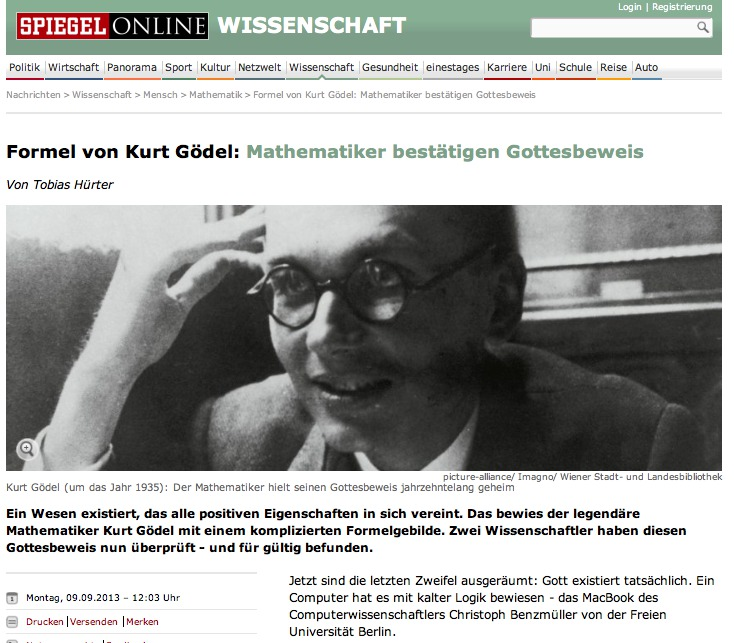
\includegraphics[width=\textwidth]{Images/News/spiegel1.jpg}}}
\onslide*<1>{\colorbox{gray}{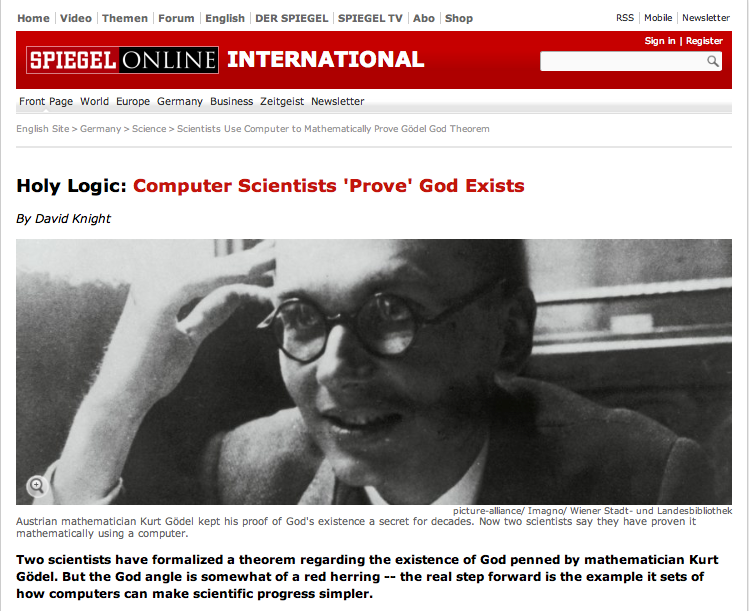
\includegraphics[width=\textwidth]{Images/News/spiegel2}}}
\vskip1em
Germany \\
- Telepolis \& Heise \\
- Spiegel Online \\
- FAZ \\
- Die Welt \\
- Berliner Morgenpost \\
- Hamburger Abendpost \\
- \ldots \\
}
%\onslide*<3>{\colorbox{gray}{
\includegraphics[width=\textwidth]{Images/News/welt}}}
\end{minipage} \hfill
%
\begin{minipage}{.3\textwidth}
Austria \\
- Die Presse \\
- Wiener Zeitung \\
- ORF \\
- \ldots \\

Italy \\
- Repubblica \\
- Ilsussidario \\
- \ldots \\

% Russia \\
% - \ldots \\

India \\
- DNA India \\
- Delhi Daily News \\
- India Today \\
- \ldots \\

US \\
- ABC News \\
- \ldots \\

International \\
- Spiegel International \\
- Yahoo Finance \\
% - CNET \\
- United Press Intl. \\
- \ldots \\
\end{minipage}

\textbf{See links at \url{https://github.com/FormalTheology/GoedelGod/tree/master/Press}}
\end{frame}



% \begin{frame}{Yes, we are in  Contact with Philosophers and Theologians \ldots} \centering
% 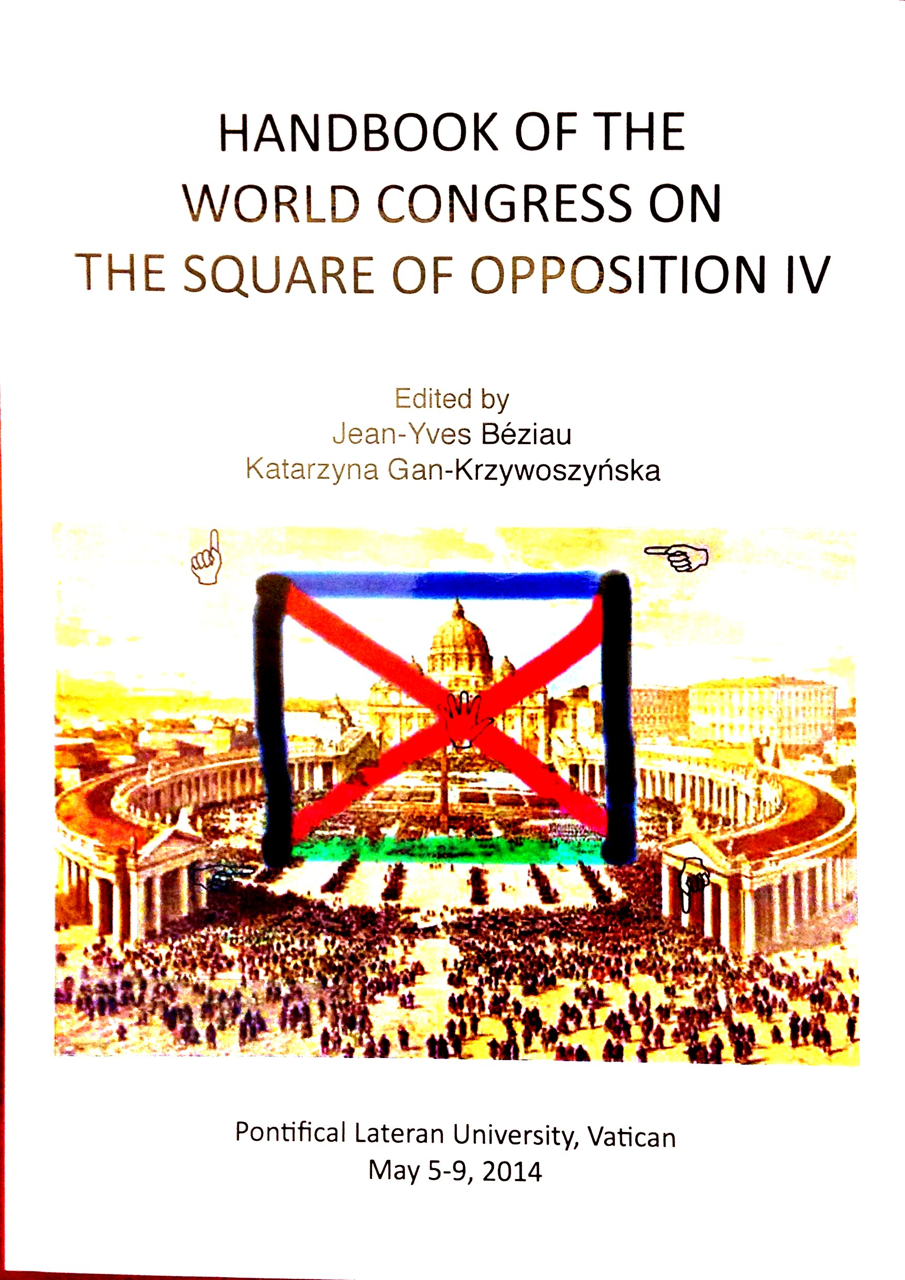
\includegraphics[width=.45\textwidth]{Images/Square.png}
% \hfill
% \includegraphics[width=.5\textheight]{Images/PhotoMitBasti.pdf}
% \end{frame}


\end{document}

\begin{transitionframe}{Images/Transitions/ReligiousSymbols(Sowlos)(CC-BY-SA)}{white}
\textbf{Part A:}

{Proof Overview (ND style)}
\end{transitionframe}




\newcommand{\phantomCOne}{
\begin{prooftree}
\AXC{$\phantom{\textbf{A3}}$} \noLine
\UIC{$\phantom{P(G)}$}
		\AXC{$\phantom{\textbf{A2}}$} \noLine
		\UIC{$\phantom{\all \varphi. \all \psi.[(P(\varphi) \wedge \nec \all x.[\varphi(x) \imp \psi(x)]) \imp P(\psi)]}$}
					\AXC{$\phantom{\textbf{A1a}}$} \noLine
					\UIC{$\phantom{\all \varphi. [P(\neg \varphi) \imp \neg P(\varphi)]}$} \noLine
				\BIC{$\phantom{\textbf{T1: } \all \varphi. [P(\varphi) \imp \pos \ex x.\varphi(x)]}$} \noLine
	\BIC{$\phantom{\textbf{C: } \pos \ex z. G(z)}$}
\end{prooftree}
}

\newcommand{\phantomTTwo}{
\begin{prooftree}
						\AXC{$\phantom{\textbf{A1b}}$} \noLine
						\UIC{$\phantom{\all \varphi. [\neg P(\varphi) \imp P(\neg \varphi)]}$}
								\AXC{$\phantom{\textbf{A4}}$} \noLine
								\UIC{$\phantom{ \all \varphi.[P(\varphi) \to \Box \; P(\varphi)]} $} \noLine
							\BIC{$\phantom{\textbf{T2: } \all y.[G(y) \imp \ess{G}{y}]}$}
									\AXC{$\phantom{\textbf{A5}}$} \noLine
									\UIC{$ \phantom{P(NE)} $} \noLine
								\BIC{$\phantom{\textbf{L1: } \ex z. G(z) \imp \nec \ex x. G(x)}$} \noLine
								\UIC{$\phantom{\pos \ex z. G(z) \imp \pos \nec \ex x. G(x)}$}
										\AXC{$\phantom{\textbf{S5}}$} \noLine
 										\UIC{$\phantom{\all \xi.[\pos \nec \xi \imp \nec \xi]}$} \noLine	
									\BIC{$\phantom{\textbf{L2: } \pos \ex z. G(z) \imp \nec \ex x. G(x)}$}
\end{prooftree}
}

\newcommand{\phantomDOne}{
$$
\phantom{
\textbf{D1: } G(x) \equiv \forall \varphi. [P(\varphi) \to \varphi(x)]}
$$
}

\newcommand{\DOne}{
$$
\textbf{D1: } G(x) \equiv \forall \varphi. [P(\varphi) \to \varphi(x)]
$$
}

\newcommand{\phantomDTwo}{
$$
\phantom{
\textbf{D2: } \ess{\varphi}{x} \equiv \varphi(x) \wedge \all \psi. (\psi(x) \imp \nec \all x. (\varphi(x) \imp \psi(x)))
}
$$
}

\newcommand{\DTwo}{
$$
\textbf{D2: } \ess{\varphi}{x} \equiv \textcolor{blue}{\varphi(x)} \wedge \all \psi. (\psi(x) \imp \nec \all x. (\varphi(x) \imp \psi(x)))
$$
}


\newcommand{\phantomDThree}{
$$
\phantom{
\textbf{D3: } NE(x) \equiv \all \varphi.[\ess{\varphi}{x} \imp \nec \ex y.\varphi(y)]
}
$$
}

\newcommand{\DThree}{
$$
\textbf{D3: } NE(x) \equiv \all \varphi.[\ess{\varphi}{x} \imp \nec \ex y.\varphi(y)]
$$
}


\begin{frame}[shrink]{Proof Overview}

\phantomDOne

\phantomDTwo

\phantomDThree

\phantomCOne

\phantomTTwo

\begin{prooftree}
\AXC{$\phantom{\textbf{C: } \pos \ex z. G(z)}$}
		\AXC{$\phantom{\textbf{L2: } \pos \ex z. G(z) \imp \nec \ex x. G(x)}$} \noLine
	\BIC{$\textbf{T3: } \nec \ex x. G(x) $}
\end{prooftree}

\end{frame}




\begin{frame}[shrink]{Proof Overview}

\phantomDOne

\phantomDTwo

\phantomDThree

\phantomCOne

\phantomTTwo

\begin{prooftree}
\AXC{$\textbf{C: } \pos \ex z. G(z)$}
		\AXC{$\phantom{\textbf{L2: } \pos \ex z. G(z) \imp \nec \ex x. G(x)}$}
	\BIC{$\textbf{T3: } \nec \ex x. G(x) $}
\end{prooftree}

\end{frame}

\newcommand{\TThree}{
\begin{prooftree}
\AXC{$\textbf{C: } \pos \ex z. G(z)$}
		\AXC{$\textbf{L2: } \pos \ex z. G(z) \imp \nec \ex x. G(x)$}
	\BIC{$\textbf{T3: } \nec \ex x. G(x) $}
\end{prooftree}	
}


\begin{frame}[shrink]{Proof Overview}

\phantomDOne

\phantomDTwo

\phantomDThree

\phantomCOne

\phantomTTwo

\TThree

\end{frame}

\begin{frame}[shrink]{Proof Overview}

\phantomDOne

\phantomDTwo

\phantomDThree

\phantomCOne

\begin{prooftree}
						\AXC{$\phantom{\textbf{A1b}}$} \noLine
						\UIC{$\phantom{\all \varphi. [\neg P(\varphi) \imp P(\neg \varphi)]}$}
								\AXC{$\phantom{\textbf{A4}}$} \noLine
								\UIC{$\phantom{ \all \varphi.[P(\varphi) \to \Box \; P(\varphi)]} $} \noLine
							\BIC{$\phantom{\textbf{T2: } \all y.[G(y) \imp \ess{G}{y}]}$}
									\AXC{$\phantom{\textbf{A5}}$} \noLine
									\UIC{$ \phantom{P(NE)} $} \noLine
								\BIC{$\phantom{\textbf{L1: } \ex z. G(z) \imp \nec \ex x. G(x)}$} \noLine
								\UIC{$\phantom{\pos \ex z. G(z) \imp \pos \nec \ex x. G(x)}$}
										\AXC{$\phantom{\textbf{S5}}$} \noLine
 										\UIC{$\phantom{\all \xi.[\pos \nec \xi \imp \nec \xi]}$} \noLine	
									\BIC{$\textbf{L2: } \pos \ex z. G(z) \imp \nec \ex x. G(x)$}
\end{prooftree}

\TThree

\end{frame}


\begin{frame}[shrink]{Proof Overview}

\phantomDOne

\phantomDTwo

\phantomDThree

\phantomCOne

\begin{prooftree}
						\AXC{$\phantom{\textbf{A1b}}$} \noLine
						\UIC{$\phantom{\all \varphi. [\neg P(\varphi) \imp P(\neg \varphi)]}$}
								\AXC{$\phantom{\textbf{A4}}$} \noLine
								\UIC{$\phantom{ \all \varphi.[P(\varphi) \to \Box \; P(\varphi)]} $} \noLine
							\BIC{$\phantom{\textbf{T2: } \all y.[G(y) \imp \ess{G}{y}]}$}
									\AXC{$\phantom{\textbf{A5}}$} \noLine
									\UIC{$ \phantom{P(NE)} $} \noLine
								\BIC{$\phantom{\textbf{L1: } \ex z. G(z) \imp \nec \ex x. G(x)}$} \noLine
								\UIC{$\phantom{\pos \ex z. G(z) \imp \pos \nec \ex x. G(x)}$}
										\AXC{$\textbf{S5}$} \dashedLine
 										\UIC{$\all \xi.[\pos \nec \xi \imp \nec \xi]$} 	
									\BIC{$\textbf{L2: } \pos \ex z. G(z) \imp \nec \ex x. G(x)$}
\end{prooftree}

\TThree

\end{frame}




\begin{frame}[shrink]{Proof Overview}

\phantomDOne

\phantomDTwo

\phantomDThree

\phantomCOne

\begin{prooftree}
						\AXC{$\phantom{\textbf{A1b}}$} \noLine
						\UIC{$\phantom{\all \varphi. [\neg P(\varphi) \imp P(\neg \varphi)]}$}
								\AXC{$\phantom{\textbf{A4}}$} \noLine
								\UIC{$\phantom{ \all \varphi.[P(\varphi) \to \Box \; P(\varphi)]} $} \noLine
							\BIC{$\phantom{\textbf{T2: } \all y.[G(y) \imp \ess{G}{y}]}$}
									\AXC{$\phantom{\textbf{A5}}$} \noLine
									\UIC{$ \phantom{P(NE)} $} \noLine
								\BIC{$\phantom{\textbf{L1: } \ex z. G(z) \imp \nec \ex x. G(x)}$} \noLine
								\UIC{$\pos \ex z. G(z) \imp \pos \nec \ex x. G(x)$}
										\AXC{$\textbf{S5}$} \dashedLine
 										\UIC{$\all \xi.[\pos \nec \xi \imp \nec \xi]$} 	
									\BIC{$\textbf{L2: } \pos \ex z. G(z) \imp \nec \ex x. G(x)$}
\end{prooftree}

\TThree

\end{frame}




\begin{frame}[shrink]{Proof Overview}

\phantomDOne

\phantomDTwo

\phantomDThree

\phantomCOne

\begin{prooftree}
						\AXC{$\phantom{\textbf{A1b}}$} \noLine
						\UIC{$\phantom{\all \varphi. [\neg P(\varphi) \imp P(\neg \varphi)]}$}
								\AXC{$\phantom{\textbf{A4}}$} \noLine
								\UIC{$\phantom{ \all \varphi.[P(\varphi) \to \Box \; P(\varphi)]} $} \noLine
							\BIC{$\phantom{\textbf{T2: } \all y.[G(y) \imp \ess{G}{y}]}$}
									\AXC{$\phantom{\textbf{A5}}$} \noLine
									\UIC{$ \phantom{P(NE)} $} \noLine
								\BIC{$\textbf{L1: } \ex z. G(z) \imp \nec \ex x. G(x)$} 
								\UIC{$\pos \ex z. G(z) \imp \pos \nec \ex x. G(x)$}
										\AXC{$\textbf{S5}$} \dashedLine
 										\UIC{$\all \xi.[\pos \nec \xi \imp \nec \xi]$} 	
									\BIC{$\textbf{L2: } \pos \ex z. G(z) \imp \nec \ex x. G(x)$}
\end{prooftree}

\TThree

\end{frame}



\begin{frame}[shrink]{Proof Overview}

\DOne

\phantomDTwo

\phantomDThree

\phantomCOne

\begin{prooftree}
						\AXC{$\phantom{\textbf{A1b}}$} \noLine
						\UIC{$\phantom{\all \varphi. [\neg P(\varphi) \imp P(\neg \varphi)]}$}
								\AXC{$\phantom{\textbf{A4}}$} \noLine
								\UIC{$\phantom{ \all \varphi.[P(\varphi) \to \Box \; P(\varphi)]} $} \noLine
							\BIC{$\phantom{\textbf{T2: } \all y.[G(y) \imp \ess{G}{y}]}$}
									\AXC{$\phantom{\textbf{A5}}$} \noLine
									\UIC{$ \phantom{P(NE)} $} \noLine
								\BIC{$\textbf{L1: } \ex z. G(z) \imp \nec \ex x. G(x)$} 
								\UIC{$\pos \ex z. G(z) \imp \pos \nec \ex x. G(x)$}
										\AXC{$\textbf{S5}$} \dashedLine
 										\UIC{$\all \xi.[\pos \nec \xi \imp \nec \xi]$} 	
									\BIC{$\textbf{L2: } \pos \ex z. G(z) \imp \nec \ex x. G(x)$}
\end{prooftree}

\TThree

\end{frame}


\begin{frame}[shrink]{Proof Overview}

\DOne

\phantomDTwo

\qquad
\alert{$\textbf{D3*: } NE(x) \equiv \nec \ex y. G(y)$} \only<2>{(cheating!)}

\phantomCOne

\begin{prooftree}
						\AXC{$\phantom{\textbf{A1b}}$} \noLine
						\UIC{$\phantom{\all \varphi. [\neg P(\varphi) \imp P(\neg \varphi)]}$}
								\AXC{$\phantom{\textbf{A4}}$} \noLine
								\UIC{$\phantom{ \all \varphi.[P(\varphi) \to \Box \; P(\varphi)]} $} \noLine
							\BIC{$\phantom{\textbf{T2: } \all y.[G(y) \imp \ess{G}{y}]}$}
									\AXC{$\phantom{\textbf{A5}}$} \noLine
									\UIC{$ P(NE) $}
								\BIC{$\textbf{L1: } \ex z. G(z) \imp \nec \ex x. G(x)$} 
								\UIC{$\pos \ex z. G(z) \imp \pos \nec \ex x. G(x)$}
										\AXC{$\textbf{S5}$} \dashedLine
 										\UIC{$\all \xi.[\pos \nec \xi \imp \nec \xi]$} 	
									\BIC{$\textbf{L2: } \pos \ex z. G(z) \imp \nec \ex x. G(x)$}
\end{prooftree}

\TThree

\end{frame}


\begin{frame}[shrink]{Proof Overview}

\DOne

\phantomDTwo

\qquad
\alert{$\textbf{D3*: } NE(x) \equiv \nec \ex y. G(y)$}
\qquad\qquad
$\textbf{D3: } NE(x) \equiv \all \varphi.[\ess{\varphi}{x} \imp \nec \ex y.\varphi(y)]$
\phantomCOne

\begin{prooftree}
						\AXC{$\phantom{\textbf{A1b}}$} \noLine
						\UIC{$\phantom{\all \varphi. [\neg P(\varphi) \imp P(\neg \varphi)]}$}
								\AXC{$\phantom{\textbf{A4}}$} \noLine
								\UIC{$\phantom{ \all \varphi.[P(\varphi) \to \Box \; P(\varphi)]} $} \noLine
							\BIC{$\textbf{T2: } \all y.[G(y) \imp \ess{G}{y}]$}
									\AXC{$\phantom{\textbf{A5}}$} \noLine
									\UIC{$ P(NE) $}
								\BIC{$\textbf{L1: } \ex z. G(z) \imp \nec \ex x. G(x)$} 
								\UIC{$\pos \ex z. G(z) \imp \pos \nec \ex x. G(x)$}
										\AXC{$\textbf{S5}$} \dashedLine
 										\UIC{$\all \xi.[\pos \nec \xi \imp \nec \xi]$} 	
									\BIC{$\textbf{L2: } \pos \ex z. G(z) \imp \nec \ex x. G(x)$}
\end{prooftree}

\TThree

\end{frame}


\begin{frame}[shrink]{Proof Overview}

\DOne

\phantomDTwo

\qquad
\alert{$\textbf{D3*: } NE(x) \equiv \nec \ex y. G(y)$}
\qquad\qquad
$\textbf{D3: } NE(x) \equiv \all \varphi.[\ess{\varphi}{x} \imp \nec \ex y.\varphi(y)]$
\phantomCOne

\begin{prooftree}
						\AXC{$\phantom{\textbf{A1b}}$} \noLine
						\UIC{$\phantom{\all \varphi. [\neg P(\varphi) \imp P(\neg \varphi)]}$}
								\AXC{$\phantom{\textbf{A4}}$} \noLine
								\UIC{$\phantom{ \all \varphi.[P(\varphi) \to \Box \; P(\varphi)]} $} \noLine
							\BIC{$\textbf{T2: } \all y.[G(y) \imp \ess{G}{y}]$}
									\AXC{$\textbf{A5}$} \dashedLine
									\UIC{$ P(NE) $}
								\BIC{$\textbf{L1: } \ex z. G(z) \imp \nec \ex x. G(x)$} 
								\UIC{$\pos \ex z. G(z) \imp \pos \nec \ex x. G(x)$}
										\AXC{$\textbf{S5}$} \dashedLine
 										\UIC{$\all \xi.[\pos \nec \xi \imp \nec \xi]$} 	
									\BIC{$\textbf{L2: } \pos \ex z. G(z) \imp \nec \ex x. G(x)$}
\end{prooftree}

\TThree

\end{frame}



\begin{frame}[shrink]{Proof Overview}

\DOne

\phantomDTwo

\qquad
\alert{$\textbf{D3*: } NE(x) \equiv \nec \ex y. G(y)$}
\qquad\qquad
$\textbf{D3: } NE(x) \equiv \all \varphi.[\ess{\varphi}{x} \imp \nec \ex y.\varphi(y)]$
\phantomCOne

\begin{prooftree}
						\AXC{$\phantom{\textbf{A1b}}$} \noLine
						\UIC{$\phantom{\all \varphi. [\neg P(\varphi) \imp P(\neg \varphi)]}$}
								\AXC{$\phantom{\textbf{A4}}$} \noLine
								\UIC{$\phantom{ \all \varphi.[P(\varphi) \to \Box \; P(\varphi)]} $} \noLine
							\BIC{$\textbf{T2: } \all y.[G(y) \imp \ess{G}{y}]$}
									\AXC{$\textbf{A5}$} \dashedLine
									\UIC{$ P(NE) $}
								\BIC{$\textbf{L1: } \ex z. G(z) \imp \nec \ex x. G(x)$} 
								\UIC{$\pos \ex z. G(z) \imp \pos \nec \ex x. G(x)$}
										\AXC{$\textbf{S5}$} \dashedLine
 										\UIC{$\all \xi.[\pos \nec \xi \imp \nec \xi]$} 	
									\BIC{$\textbf{L2: } \pos \ex z. G(z) \imp \nec \ex x. G(x)$}
\end{prooftree}

\TThree

\end{frame}


\newcommand{\LTwo}{
\begin{prooftree}
						\AXC{$\textbf{A1b}$} \dashedLine
						\UIC{$\all \varphi. [\neg P(\varphi) \imp P(\neg \varphi)]$}
								\AXC{$\textbf{A4}$} \dashedLine
								\UIC{$ \all \varphi.[P(\varphi) \to \Box \; P(\varphi)] $} 
							\BIC{$\textbf{T2: } \all y.[G(y) \imp \ess{G}{y}]$}
									\AXC{$\textbf{A5}$} \dashedLine
									\UIC{$ P(NE) $}
								\BIC{$\textbf{L1: } \ex z. G(z) \imp \nec \ex x. G(x)$} 
								\UIC{$\pos \ex z. G(z) \imp \pos \nec \ex x. G(x)$}
										\AXC{$\textbf{S5}$} \dashedLine
 										\UIC{$\all \xi.[\pos \nec \xi \imp \nec \xi]$} 	
									\BIC{$\textbf{L2: } \pos \ex z. G(z) \imp \nec \ex x. G(x)$}
\end{prooftree}
}


\begin{frame}[shrink]{Proof Overview}

\DOne

\DTwo

\qquad
\alert{$\textbf{D3*: } NE(x) \equiv \nec \ex y. G(y)$}
\qquad\qquad
$\textbf{D3: } NE(x) \equiv \all \varphi.[\ess{\varphi}{x} \imp \nec \ex y.\varphi(y)]$

\phantomCOne

\LTwo

\TThree

\end{frame}


\begin{frame}[shrink]{Proof Overview}

\DOne

\DTwo

\qquad
\alert{$\textbf{D3*: } NE(x) \equiv \nec \ex y. G(y)$}
\qquad\qquad
$\textbf{D3: } NE(x) \equiv \all \varphi.[\ess{\varphi}{x} \imp \nec \ex y.\varphi(y)]$

\begin{prooftree}
\AXC{$\phantom{\textbf{A3}}$} \noLine
\UIC{$\phantom{P(G)}$}
		\AXC{$\phantom{\textbf{A2}}$} \noLine
		\UIC{$\phantom{\all \varphi. \all \psi.[(P(\varphi) \wedge \nec \all x.[\varphi(x) \imp \psi(x)]) \imp P(\psi)]}$}
					\AXC{$\phantom{\textbf{A1a}}$} \noLine
					\UIC{$\phantom{\all \varphi. [P(\neg \varphi) \imp \neg P(\varphi)]}$} \noLine
				\BIC{$\phantom{\textbf{T1: } \all \varphi. [P(\varphi) \imp \pos \ex x.\varphi(x)]}$} \noLine
	\BIC{$\textbf{C: } \pos \ex z. G(z)$}
\end{prooftree}

\LTwo

\TThree

\end{frame}


\begin{frame}[shrink]{Proof Overview}

\DOne

\DTwo

\qquad
\alert{$\textbf{D3*: } NE(x) \equiv \nec \ex y. G(y)$}
\qquad\qquad
$\textbf{D3: } NE(x) \equiv \all \varphi.[\ess{\varphi}{x} \imp \nec \ex y.\varphi(y)]$

\begin{prooftree}
\AXC{$\phantom{\textbf{A3}}$} \noLine
\UIC{$P(G)$}
		\AXC{$\phantom{\textbf{A2}}$} \noLine
		\UIC{$\phantom{\all \varphi. \all \psi.[(P(\varphi) \wedge \nec \all x.[\varphi(x) \imp \psi(x)]) \imp P(\psi)]}$}
					\AXC{$\phantom{\textbf{A1a}}$} \noLine
					\UIC{$\phantom{\all \varphi. [P(\neg \varphi) \imp \neg P(\varphi)]}$} \noLine
				\BIC{$\phantom{\textbf{T1: } \all \varphi. [P(\varphi) \imp \pos \ex x.\varphi(x)]}$} 
	\BIC{$\textbf{C: } \pos \ex z. G(z)$}
\end{prooftree}

\LTwo

\TThree

\end{frame}


\begin{frame}[shrink]{Proof Overview}

\DOne

\DTwo

\qquad
\alert{$\textbf{D3*: } NE(x) \equiv \nec \ex y. G(y)$}
\qquad\qquad
$\textbf{D3: } NE(x) \equiv \all \varphi.[\ess{\varphi}{x} \imp \nec \ex y.\varphi(y)]$

\begin{prooftree}
\AXC{$\textbf{A3}$} \dashedLine
\UIC{$P(G)$}
		\AXC{$\phantom{\textbf{A2}}$} \noLine
		\UIC{$\phantom{\all \varphi. \all \psi.[(P(\varphi) \wedge \nec \all x.[\varphi(x) \imp \psi(x)]) \imp P(\psi)]}$}
					\AXC{$\phantom{\textbf{A1a}}$} \noLine
					\UIC{$\phantom{\all \varphi. [P(\neg \varphi) \imp \neg P(\varphi)]}$} \noLine
				\BIC{$\phantom{\textbf{T1: } \all \varphi. [P(\varphi) \imp \pos \ex x.\varphi(x)]}$} 
	\BIC{$\textbf{C: } \pos \ex z. G(z)$}
\end{prooftree}

\LTwo

\TThree

\end{frame}



\begin{frame}[shrink]{Proof Overview}

\DOne

\DTwo

\qquad
\alert{$\textbf{D3*: } NE(x) \equiv \nec \ex y. G(y)$}
\qquad\qquad
$\textbf{D3: } NE(x) \equiv \all \varphi.[\ess{\varphi}{x} \imp \nec \ex y.\varphi(y)]$

\begin{prooftree}
\AXC{$\textbf{A3}$} \dashedLine
\UIC{$P(G)$}
		\AXC{$\phantom{\textbf{A2}}$} \noLine
		\UIC{$\phantom{\all \varphi. \all \psi.[(P(\varphi) \wedge \nec \all x.[\varphi(x) \imp \psi(x)]) \imp P(\psi)]}$}
					\AXC{$\phantom{\textbf{A1a}}$} \noLine
					\UIC{$\phantom{\all \varphi. [P(\neg \varphi) \imp \neg P(\varphi)]}$} \noLine
				\BIC{$\textbf{T1: } \all \varphi. [P(\varphi) \imp \pos \ex x.\varphi(x)]$} 
	\BIC{$\textbf{C: } \pos \ex z. G(z)$}
\end{prooftree}

\LTwo

\TThree

\end{frame}



\begin{frame}[shrink]{Proof Overview}

\DOne

\DTwo

\qquad
\alert{$\textbf{D3*: } NE(x) \equiv \nec \ex y. G(y)$}
\qquad\qquad
$\textbf{D3: } NE(x) \equiv \all \varphi.[\ess{\varphi}{x} \imp \nec \ex y.\varphi(y)]$

\begin{prooftree}
\AXC{$\textbf{A3}$} \dashedLine
\UIC{$P(G)$}
		\AXC{$\textbf{A2}$} \dashedLine
		\UIC{$\all \varphi. \all \psi.[(P(\varphi) \wedge \nec \all x.[\varphi(x) \imp \psi(x)]) \imp P(\psi)]$}
					\AXC{$\textbf{A1a}$} \dashedLine
					\UIC{$\all \varphi. [P(\neg \varphi) \imp \neg P(\varphi)]$}
				\BIC{$\textbf{T1: } \all \varphi. [P(\varphi) \imp \pos \ex x.\varphi(x)]$} 
	\BIC{$\textbf{C: } \pos \ex z. G(z)$}
\end{prooftree}

\LTwo

\TThree

\end{frame}



\begin{frame}[shrink]{Proof Overview}

$$
\textbf{D1: } G(x) \equiv \forall \varphi. [P(\varphi) \to \varphi(x)]
$$

$$
\textbf{D2: } \ess{\varphi}{x} \equiv \varphi(x) \wedge \all \psi. (\psi(x) \imp \nec \all x. (\varphi(x) \imp \psi(x)))
$$

$$
\textbf{D3: } NE(x) \equiv \all \varphi.[\ess{\varphi}{x} \imp \nec \ex y.\varphi(y)]
$$

\begin{prooftree}
\AXC{$\textbf{A3}$} \dashedLine
\UIC{$P(G)$}
		\AXC{$\textbf{A2}$} \dashedLine
		\UIC{$\all \varphi. \all \psi.[(P(\varphi) \wedge \nec \all x.[\varphi(x) \imp \psi(x)]) \imp P(\psi)]$}
					\AXC{$\textbf{A1a}$} \dashedLine
					\UIC{$\all \varphi. [P(\neg \varphi) \imp \neg P(\varphi)]$} \doubleLine
				\BIC{$\textbf{T1: } \all \varphi. [P(\varphi) \imp \pos \ex x.\varphi(x)]$} \doubleLine
	\BIC{$\textbf{C: } \pos \ex z. G(z)$}
\end{prooftree}





\begin{prooftree}
						\AXC{$\textbf{A1b}$} \dashedLine
						\UIC{$\all \varphi. [\neg P(\varphi) \imp P(\neg \varphi)]$}
								\AXC{$\textbf{A4}$} \dashedLine
								\UIC{$ \all \varphi.[P(\varphi) \to \Box \; P(\varphi)] $} \doubleLine
							\BIC{$\textbf{T2: } \all y.[G(y) \imp \ess{G}{y}]$}
									\AXC{$\textbf{A5}$} \dashedLine
									\UIC{$ P(NE) $} \doubleLine
								\BIC{$\textbf{L1: } \ex z. G(z) \imp \nec \ex x. G(x)$} \doubleLine
								\UIC{$\pos \ex z. G(z) \imp \pos \nec \ex x. G(x)$}
										\AXC{$\textbf{S5}$} \dashedLine
 										\UIC{$ \all \xi.[\pos \nec \xi \imp \nec \xi]$} \doubleLine	
									\BIC{$\textbf{L2: } \pos \ex z. G(z) \imp \nec \ex x. G(x)$}
\end{prooftree}

\begin{prooftree}
\AXC{$\textbf{C: } \pos \ex z. G(z)$}
		\AXC{$\textbf{L2: } \pos \ex z. G(z) \imp \nec \ex x. G(x)$} \doubleLine
	\BIC{$\textbf{T3: } \nec \ex x. G(x) $}
\end{prooftree}

\end{frame}

% \begin{transitionframe}{Images/Transitions/RioChrist3}
\textbf{Part A:}

Informal Proof and Natural Deduction Proof
\end{transitionframe}




\begin{frame}{G\"odel's Manuscript (1970)}
\bigskip

\begin{changemargin}{-1.2cm}{-1.2cm}
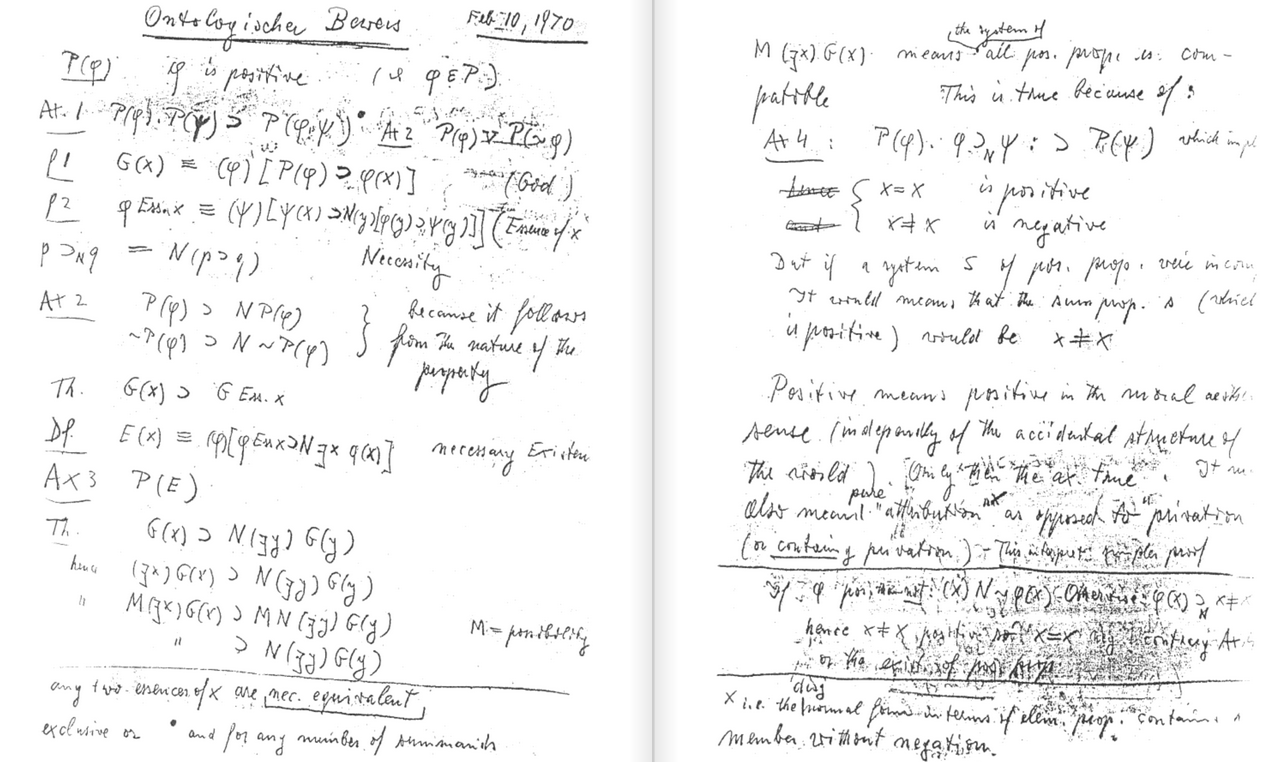
\includegraphics[width=13cm]{Images/Manuscript.png}
\end{changemargin}
\end{frame}

\begin{frame}{Scott's Version of G\"odel's Axioms, Definitions and Theorems}
\begin{changemargin}{-0.9cm}{-0.8cm}
\colorbox{black}{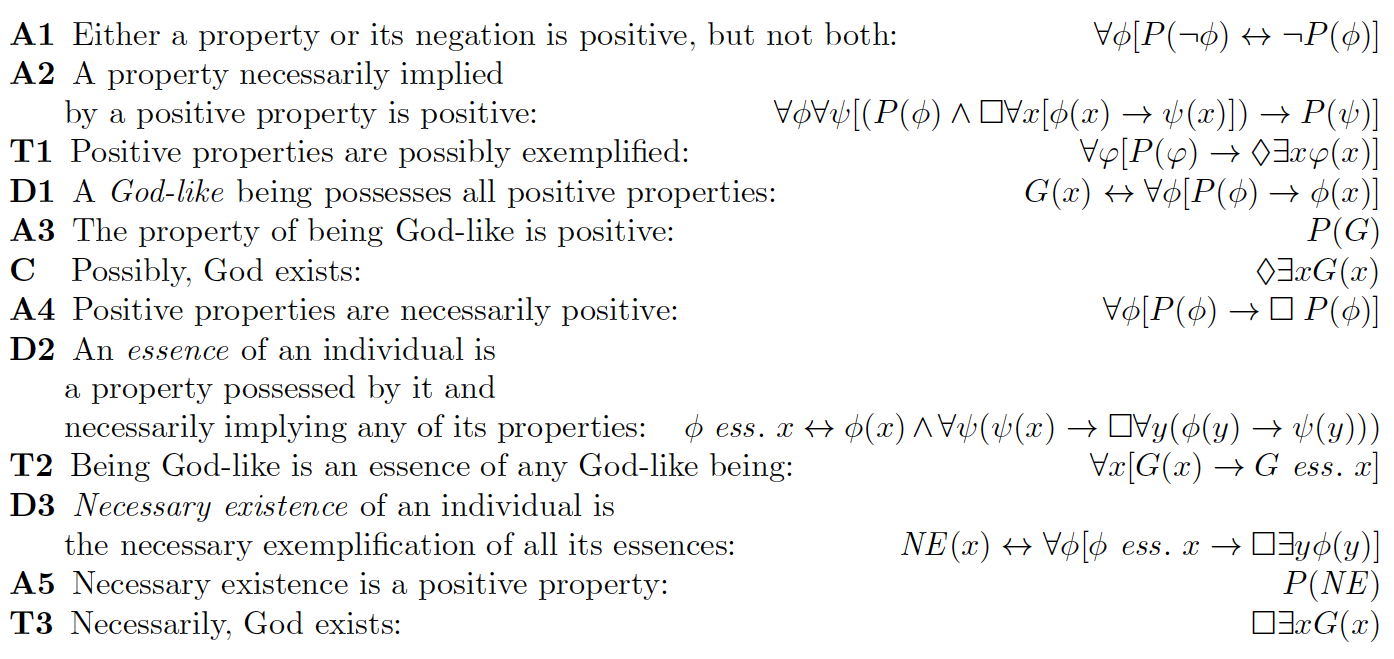
\includegraphics[width=12.4cm]{Images/ScottsScriptGrab.png}}
\end{changemargin}
\end{frame}


\begin{frame}[shrink]{Proof Overview}

$$
\textbf{D1: } G(x) \equiv \forall \varphi. [P(\varphi) \to \varphi(x)]
$$

$$
\textbf{D2: } \ess{\varphi}{x} \equiv \varphi(x) \wedge \all \psi. (\psi(x) \imp \nec \all x. (\varphi(x) \imp \psi(x)))
$$

$$
\textbf{D3: } E(x) \equiv \all \varphi.[\ess{\varphi}{x} \imp \nec \ex y.\varphi(y)]
$$

\begin{prooftree}
\AXC{$\textbf{A3}$} \dashedLine
\UIC{$P(G)$}
		\AXC{$\textbf{A2}$} \dashedLine
		\UIC{$\all \varphi. \all \psi.[(P(\varphi) \wedge \nec \all x.[\varphi(x) \imp \psi(x)]) \imp P(\psi)]$}
					\AXC{$\textbf{A1a}$} \dashedLine
					\UIC{$\all \varphi. [P(\neg \varphi) \imp \neg P(\varphi)]$} \doubleLine
				\BIC{$\textbf{T1: } \all \varphi. [P(\varphi) \imp \pos \ex x.\varphi(x)]$} \doubleLine
	\BIC{$\textbf{C1: } \pos \ex x. G(x)$}
\end{prooftree}



\begin{prooftree}
						\AXC{$\textbf{A1b}$} \dashedLine
						\UIC{$\all \varphi. [\neg P(\varphi) \imp P(\neg \varphi)]$}
								\AXC{$\textbf{A4}$} \dashedLine
								\UIC{$ \all \varphi.[P(\varphi) \to \Box \; P(\varphi)] $} \doubleLine
							\BIC{$\textbf{T2: } \all y.[G(y) \imp \ess{G}{y}]$}
									\AXC{$\textbf{A5}$} \dashedLine
									\UIC{$ P(E) $} \doubleLine
								\BIC{$\textbf{L1: } \ex z. G(z) \imp \nec \ex x. G(x)$} \doubleLine
								\UIC{$\pos \ex z. G(z) \imp \pos \nec \ex x. G(x)$}
										\AXC{$\textbf{S5}$} \dashedLine
 										\UIC{$ \all \xi.[\pos \nec \xi \imp \nec \xi]$} \doubleLine	
									\BIC{$\textbf{L2: } \pos \ex z. G(z) \imp \nec \ex x. G(x)$}
\end{prooftree}

\begin{prooftree}
\AXC{$\textbf{C1: } \pos \ex x. G(x)$}
		\AXC{$\textbf{L2: } \pos \ex z. G(z) \imp \nec \ex x. G(x)$} \doubleLine
	\BIC{$\textbf{T3: } \nec \ex x. G(x) $}
\end{prooftree}

\end{frame}

\begin{frame}[shrink]{Natural Deduction Calculus}

\begin{unnamedCalculus}

\vspace{1em}

\s\s
\infer[\vee_E]{C}{A \vee B & \infer*{C}{\infer{A}{}} & \infer*{C}{\infer{B}{}}}
\s\s
\infer[\wedge_I]{A \wedge B}{A & B}
\s\s
\infer[\imp_I^n]{A \imp B}{ \infer*{B}{\infer[n]{A}{}} }

\vspace{2em}

\s\s
\infer[\vee_{I_1}]{A \vee B}{A}
\s\s
\infer[\wedge_{E_1}]{A}{A \wedge B}
\s\s
\infer[\imp_I]{A \imp B}{ B }

\vspace{2em}

\s\s
\infer[\vee_{I_2}]{A \vee B}{B}
\s\s
\infer[\wedge_{E_2}]{B}{A \wedge B}
\s\s
\infer[\imp_E]{B}{A & A \imp B}

\vspace{2em}

\s
\infer[\all_I]{\all x. A[x]}{ A[\alpha] }
\s
\infer[\all_E]{A[t]}{ \all x. A[x] }
\s\s
\infer[\ex_I]{\ex x. A[x]}{ A[t] }
\s
\infer[\ex_E]{A[\beta]}{ \ex x. A[x] }

\vspace{1em}

\s\s\s\s
$\neg A \equiv A \imp \bot$ 
\s\s\s 
\alert{\infer[\neg\neg_E]{A}{\neg\neg A}}

\vspace{1em}

\end{unnamedCalculus}

\end{frame}



\begin{frame}[shrink]{Natural Deduction Calculus}{Rules for Modalities}

\begin{unnamedCalculus}

\vspace{1em}

\s\s\s\s
\infer[\nec_I]{\nec A}{\alpha: \fbox{\infer*{A}{}} }
\s\s\s\s\s
\infer[\nec_E]{t: \fbox{ \infer*{}{A} }  }{\nec A}

\vspace{2em}

\s\s\s\s
\infer[\pos_I]{\pos A}{t: \fbox{\infer*{A}{}} }
\s\s\s\s\s
\infer[\pos_E]{\beta: \fbox{ \infer*{}{A} }  }{\pos A}

\vspace{2em}

\alert{$$\pos A \equiv \neg \nec \neg A$$}

\vspace{1em}

\end{unnamedCalculus}

\end{frame}



\begin{frame}{Natural Deduction Proofs}{T1 and C1}
\begin{prooftree}
        \AXC{\textbf{A2}} \dashedLine
        \UIC{$ \all \varphi. \all \psi.[(P(\varphi) \wedge \nec \all x.[\varphi(x) \imp \psi(x)]) \imp P(\psi)]$} \RightLabel{$\all_E$}
        \UIC{$ \all \psi.[(P(\rho) \wedge \nec \all x.[\rho(x) \imp \psi(x)]) \imp P(\psi)]$} \RightLabel{$\all_E$}
        \UIC{$(P(\rho) \wedge \nec \all x.[\rho(x) \imp \neg \rho(x)]) \imp P(\neg \rho)$} \doubleLine
        \UIC{$(P(\rho) \wedge \nec \all x.[\neg \rho(x)]) \imp P(\neg \rho)$}
                        \AXC{\textbf{A1a}} \dashedLine
                        \UIC{$\all \varphi.[ P(\neg \varphi) \imp \neg P(\varphi) ]$} \RightLabel{$\all_E$}
                        \UIC{$ P(\neg \rho) \imp \neg P(\rho) $} \doubleLine
                 \BIC{$ (P(\rho) \wedge \nec \all x.[\neg \rho(x)]) \imp \neg P(\rho) $} \doubleLine
                 \UIC{$ P(\rho) \imp \pos \ex x.\rho(x) $} \RightLabel{$\all_I$}
                 \UIC{$\all \varphi.[ P(\varphi) \imp \pos \ex x.\varphi(x) ] $}
\end{prooftree}

\begin{prooftree}
\AXC{\textbf{A3}} \dashedLine
\UIC{$P(G)$}
                 \AXC{\textbf{T1}} \dashedLine
                 \UIC{$\all \varphi.[ P(\varphi) \imp \pos \ex x.\varphi(x) ]$} \RightLabel{$\all_E $}
                 \UIC{$ P(G) \imp \pos \ex x.G(x) $} \RightLabel{$\imp_E$}
    \BIC{$\pos \ex x. G(x)$}
\end{prooftree}
\end{frame}



\begin{frame}{Natural Deduction Proofs}{T2 (Partial)}
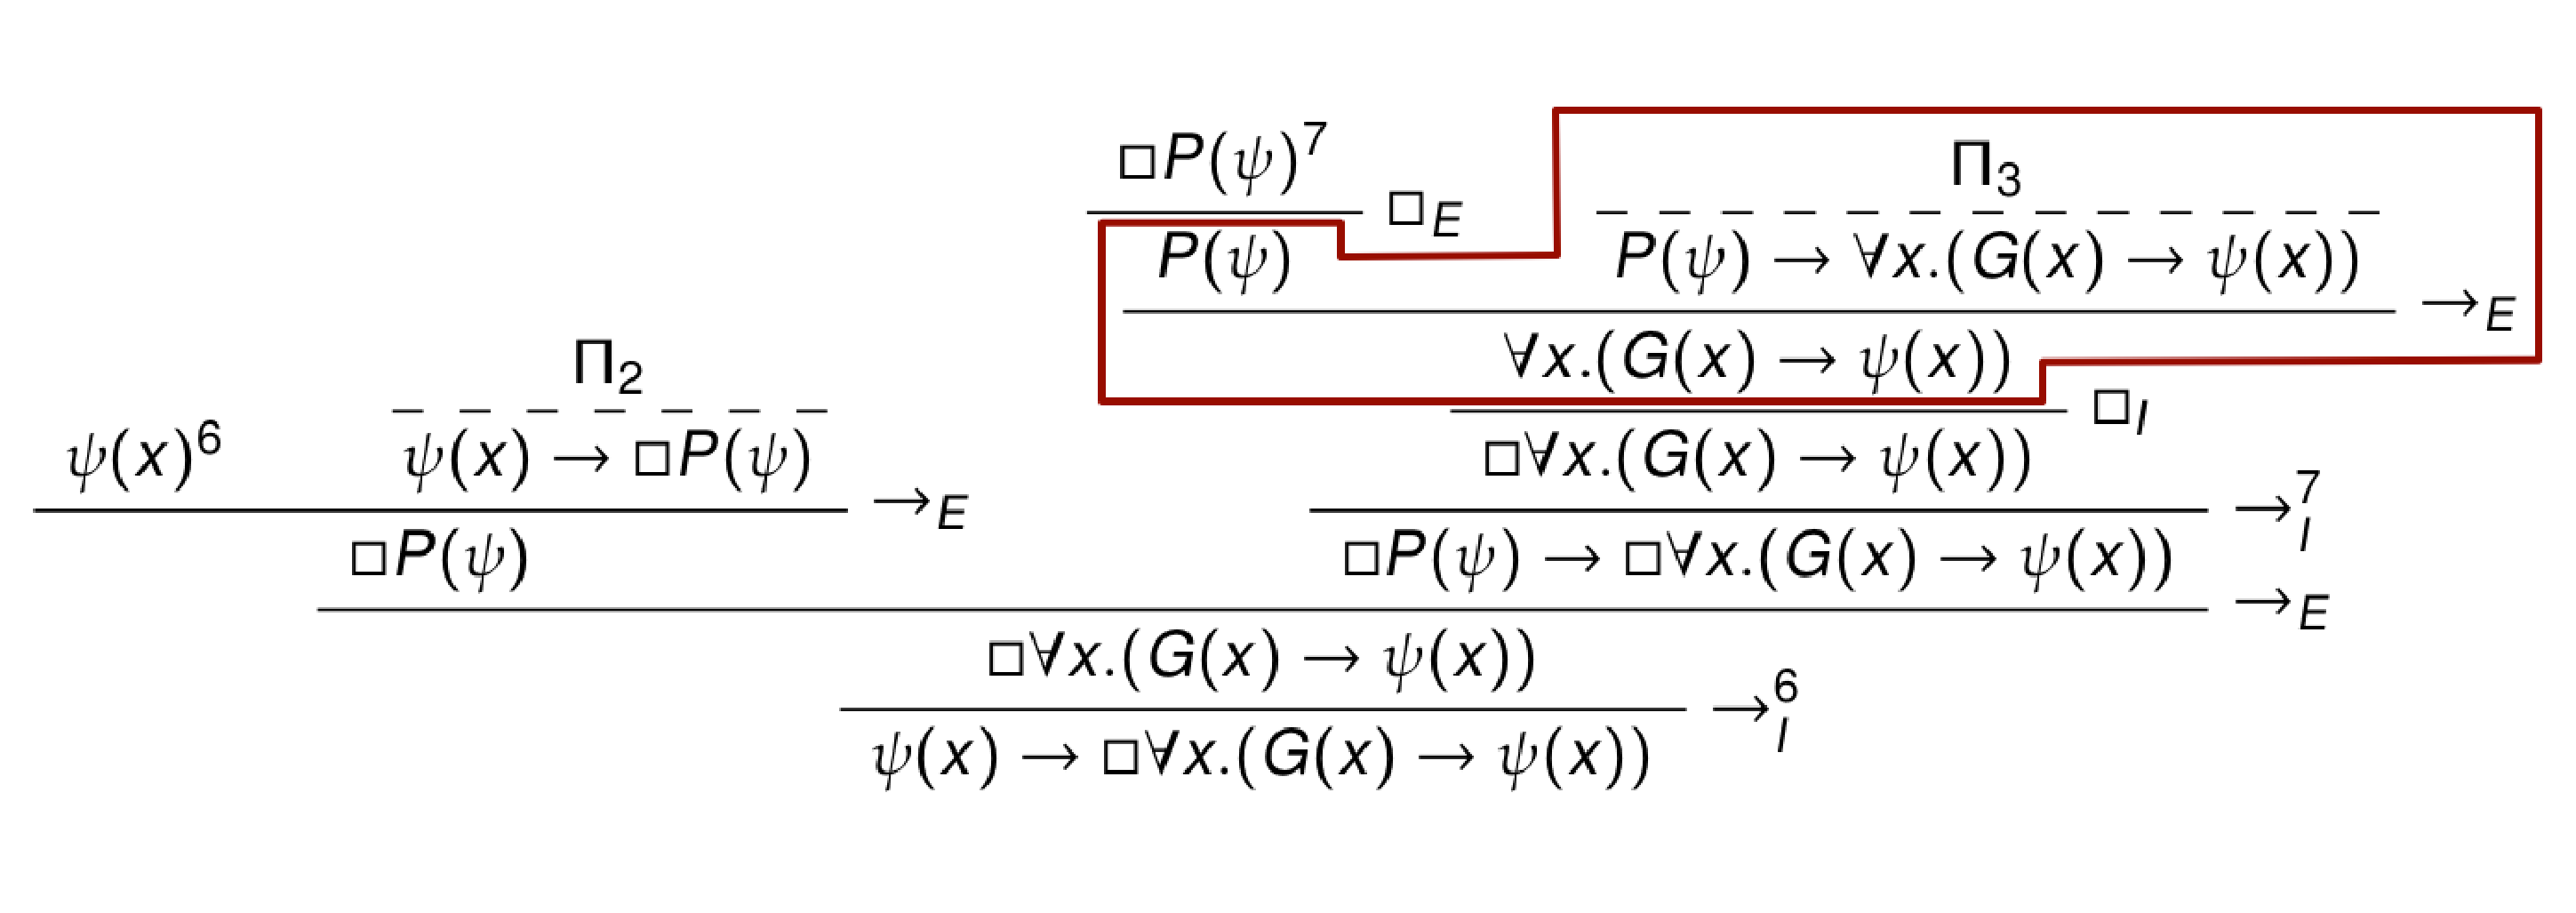
\includegraphics[scale=0.22]{Images/ProofOfT2Boxed.pdf}
\end{frame}


% \begin{transitionframe}{}
\textbf{Part B:} \\[.5em]
\quad Formalization: \hfill in classical higher-order logic (\textcolor{black}{HOL}) \\
\quad Automation: \hfill theorem provers \textsc{Leo-II} and \textsc{Satallax} \\ 
\quad Consistency: \hfill model finder \textsc{Nitpick (Nitrox)} \\
\end{transitionframe}

\begin{frame}{Formalization in HOL} \large

\hskip-1em Challenge: \hfill No provers for \emph{Higher-order
  Quantified Modal
  Logic\/} (\textcolor{red}{QML}) \\[1em]

\hskip-1em Our solution: \hfill Embedding in \emph{Higher-order Classical
  Logic\/} (\textcolor{blue}{HOL}) \\
\, \hfill Then use existing \textcolor{blue}{HOL} theorem provers for reasoning in \textcolor{red}{QML} \\
\,\hfill {\small [Benzm\"ullerPaulson, Logica Universalis, 2013]}
\\[2em]

Previous empiricial findings:  \\[.5em]
\,\hfill Embedding of  \emph{First-order Modal Logic} in HOL works well 

\,\hfill {\small [Benzm\"ullerOttenRaths, ECAI, 2012]} \\
\,\hfill {\small [Benzm\"uller, LPAR, 2013]}
\end{frame}



\begin{frame}{Formalization in HOL} \large

\hskip-1em\textcolor{red}{QML} \hfill
$\begin{array}{lll}\textcolor{red}{\varphi,\psi} & ::= &
  \textcolor{red}{\ldots}  \mid \textcolor{red}{\neg
    \varphi} \mid \textcolor{red}{\varphi \wedge \psi} \mid
  \textcolor{red}{\varphi \imp \psi}  \mid \textcolor{red}{\Box
    \varphi} \mid \textcolor{red}{\Diamond \varphi}  \mid
  \textcolor{red}{\forall {x}\, \varphi} \mid
  \textcolor{red}{\exists {x}\, \varphi} 
\mid \textcolor{red}{\forall {P}\, \varphi} \end{array}$ \\[1em]


\begin{itemize}
\item Kripke style semantics (possible world semantics)\\[2em]
\end{itemize}



\hskip-1em\textcolor{blue}{HOL}\hfill 
$\begin{array}{lll}
\textcolor{blue}{s,t} & ::= & \textcolor{blue}{C}  \mid
\textcolor{blue}{x \mid \lambda{x} s} \mid \textcolor{blue}{s\, t}
\mid \textcolor{blue}{\neg s} \mid \textcolor{blue}{s \vee t} \mid
\textcolor{blue}{\forall {x}\, t} 
\end{array}$ \\[1em]

\begin{itemize}
\item meanwhile very well understood
\item Henkin semantics vs. standard semantics
\item various theorem provers do exists \\[.5em]
  \quad interactive: \hfill Isabelle/HOL, HOL4, Hol Light, Coq/HOL, PVS,
  \ldots \\[.5em]
  \quad automated: \hfill TPS, LEO-II, Satallax, Nitpick, Isabelle/HOL, \ldots \\
\end{itemize}


\end{frame}


\begin{frame}{Formalization in HOL}\large

\hskip-1em\textcolor{red}{QML} \hfill
$\begin{array}{lll}\textcolor{red}{\varphi,\psi} & ::= &
  \textcolor{red}{\ldots}  \mid \textcolor{red}{\neg
    \varphi} \mid \textcolor{red}{\varphi \wedge \psi} \mid
  \textcolor{red}{\varphi \imp \psi}  \mid \textcolor{red}{\Box
    \varphi} \mid \textcolor{red}{\Diamond \varphi}  \mid
  \textcolor{red}{\forall {x}\, \varphi} \mid
  \textcolor{red}{\exists {x}\, \varphi} 
\mid \textcolor{red}{\forall {P}\, \varphi} \end{array}$ \\[1.5em]

\hskip-1em\textcolor{blue}{HOL}\hfill 
$\begin{array}{lll}
\textcolor{blue}{s,t} & ::= & \textcolor{blue}{C}  \mid
\textcolor{blue}{x \mid \lambda{x} s} \mid \textcolor{blue}{s\, t}
\mid \textcolor{blue}{\neg s} \mid \textcolor{blue}{s \vee t} \mid
\textcolor{blue}{\forall {x}\, t} 
\end{array}$ \\[1.5em]


\hskip-1em\textcolor{red}{QML} in \textcolor{blue}{HOL}: \quad \textcolor{red}{QML}
formulas $\textcolor{red}{\varphi}$ are mapped to
\textcolor{blue}{HOL} predicates $\textcolor{red}{\varphi_{\worldtype\typearrow o}}$

\begin{center}
\fcolorbox{blue}{white}{
$\begin{array}{lcl} 
    \textcolor{red}{\mnot} & = & \textcolor{blue}{
      \lambda{\varphi_{\worldtype\typearrow o}}\lambda{s_\worldtype}\neg \varphi s} \\ 
    \textcolor{red}{\mand} & = & \textcolor{blue}{ 
      \lambda{\varphi_{\worldtype\typearrow o}}
      \lambda{\psi_{\worldtype\typearrow o}} \lambda{s_\worldtype}
      (\varphi s \wedge \psi s)} \\ 
    \textcolor{red}{\imp} & = & \textcolor{blue}{ 
      \lambda{\varphi_{\worldtype\typearrow o}}
      \lambda{\psi_{\worldtype\typearrow o}} \lambda{s_\worldtype}
      (\neg \varphi s \vee \psi s)} \\ 
    \textcolor{red}{\Box} & = & \textcolor{blue}{ 
      \lambda{\varphi_{\worldtype\typearrow o}} \lambda{s_\worldtype}
      \forall {u_\worldtype}\, (\neg r s u \vee
      \varphi u)} \\ 
    \textcolor{red}{\Diamond} & = & \textcolor{blue}{ 
      \lambda{\varphi_{\worldtype\typearrow o}} \lambda{s_\worldtype}
      \exists {u_\worldtype}\, (r s u \wedge
      \varphi u)} \\ 
    \textcolor{red}{\forall} & = & \textcolor{blue}{ 
      \lambda{h_{\mu\typearrow(\worldtype \typearrow o)}}
      \lambda{s_\worldtype} \forall {d_\indtype} \, h d s} \\
    \textcolor{red}{\exists} & = & \textcolor{blue}{ 
      \lambda{h_{\mu\typearrow(\worldtype \typearrow o)}}
      \lambda{s_\worldtype} \exists {d_\indtype} \, h d s} \\
    \textcolor{red}{\forall} & = & \textcolor{blue}{ 
      \lambda{H_{(\mu\typearrow(\worldtype \typearrow o))\typearrow(\worldtype \typearrow o)}}
      \lambda{s_\worldtype} \forall {d_\indtype} \, H d s} \\
    \\
      \text{\textcolor{brown}{valid}} & = & \textcolor{blue}{
        \lambda{\varphi_{\worldtype\typearrow o}} \all{w_\worldtype}
        \varphi w}
\end{array}$
}  \quad \textcolor{blue}{Ax} 
\vskip1em
\end{center}
\quad The equations in \textcolor{blue}{Ax} are given as axioms to the \textcolor{blue}{HOL} provers! \\
\quad \textcolor{gray}{\small (Remark: We are here dealing with constant domain quantification.)}

\end{frame}



\begin{frame}{Formalization in HOL} \large

\hskip-1em Example \\[.5em]

 \textcolor{red}{QML} formula  \hfill \textcolor{red}{$\Diamond \exists x G(x)$}

 \textcolor{red}{QML} formula in \textcolor{blue}{HOL}  \hfill $\text{\textcolor{brown}{valid}}\, \textcolor{red}{(\Diamond \exists x G(x))_{\worldtype\typearrow o}}$

expansion, $\beta\eta$-conversion \hfill $\textcolor{blue}{\forall
  w_\worldtype\textcolor{red}{(\Diamond \exists x
    G(x))_{\worldtype\typearrow o}}\, w}$ 

expansion, $\beta\eta$-conversion \hfill $\textcolor{blue}{\forall
  w_\worldtype \exists {u_\worldtype} (r w u \wedge
      \textcolor{red}{(\exists x G(x))_{\worldtype\typearrow o}} u)}$ 

% expansion, $\beta\eta$-conversion \hfill $\textcolor{blue}{\forall
%   w_\worldtype \exists {u_\worldtype} (r w u \wedge
%       \exists x \textcolor{red}{G(x)_{\worldtype\typearrow o}} u)}$ 

expansion, $\beta\eta$-conversion \hfill $\textcolor{blue}{\forall
  w_\worldtype \exists {u_\worldtype} (r w u \wedge
      \exists x G x u)}$ \\[1em]
\pause
\vfill
\begin{block}{What are we doing?}
\vskip.5em
In order to prove that $\textcolor{red}{\varphi}$ is valid in \textcolor{red}{QML}, \\
--> we instead prove that 
$\text{\textcolor{brown}{valid}}\,
\textcolor{red}{\varphi_{\worldtype\typearrow o}}$ can be derived
from \textcolor{blue}{Ax} in \textcolor{blue}{HOL}. \\[1em]

This can be done with interactive or automated \textcolor{blue}{HOL} theorem provers.
\end{block}
\pause
\vfill
\hskip-1em Expansion: \hfill user or prover may flexibly choose expansion depth \\[.5em]

\end{frame}


\begin{frame}{Automated Theorem Provers and Model Finders for HOL}
\includegraphics[width=1.05\textwidth]{HOLProversGrab}
\end{frame}


\begin{frame}{Proof Automation and Consistency Checking: Demo!} \large
\colorbox{gray}{\includegraphics[width=\textwidth]{DemoGrap}} 
\vfill 
Provers are called remotely in Miami --- no local installation needed!
\end{frame}


% 
\begin{frame}{Coq Proof}{Demo} \small
\begin{itemize}
\item Goal: verification of the natural deduction proof
\begin{itemize}
\item Step-by-step formalization
\item Almost no automation (intentionally!)
\end{itemize}
%
\item Interesting facts to note:
\begin{itemize}
\item Embedding is transparent to the user
\item Embedding gives labeled calculus for free
\end{itemize}
\end{itemize}
\end{frame}


% 
\begin{transitionframe}{} \Large \centering
\textbf{Part D:} \\[.5em]
\quad automation \& verification: proof assistant \textsc{Isabelle} \\[2em]
\end{transitionframe}

\begin{frame}{} \Large \centering
\vskip.5em
\colorbox{gray}{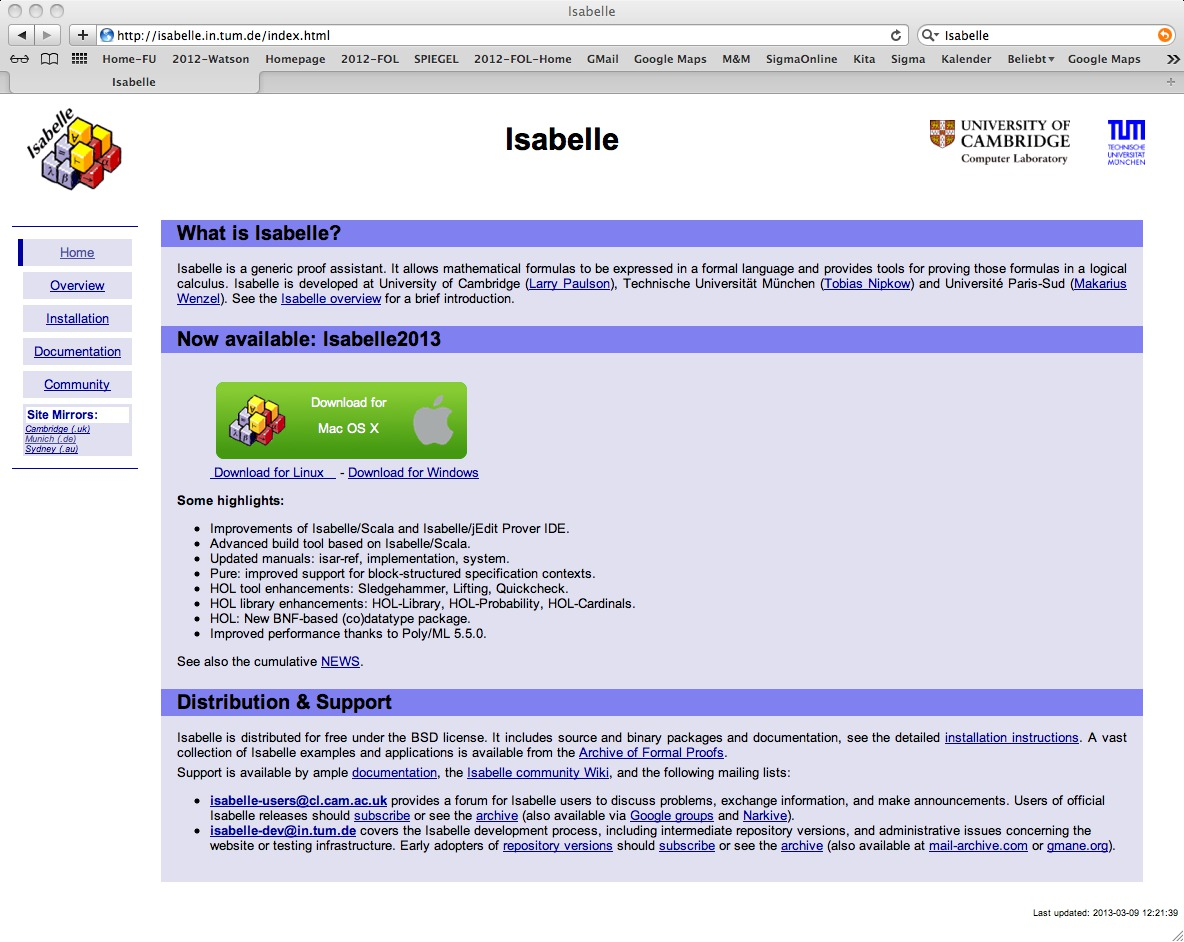
\includegraphics[width=\textwidth]{IsabelleGrab}} 
\end{frame}


\begin{frame}{Automation \& Verification in Proof Assistant \textsc{Isabelle/HOL}} \large
Isabelle/HOL   (Cambridge University/TU Munich)
\begin{itemize}
\item HOL instance of the generic \textsc{Isabelle} proof assistant
\item User interaction and proof automation 
\item Automation is supported by \textsc{Sledgehammer} tool
\item Verification of the proofs in \textsc{Isabelle/HOL}'s small proof kernel
\end{itemize}
\vfill
What we did?
\begin{itemize}
\item Proof automation of G\"odel's proof script (Scott version)
\item \textsc{Sledgehammer} makes calls to remote THF provers in Miami
\item These calls the suggest respective calls to the \textsc{Metis} prover
\item \textsc{Metis} proofs are verified in \textsc{Isabelle/HOL}'s proof kernel
\end{itemize}
\vfill
See the handout (generated from the Isabelle source file).
\end{frame}


\begin{frame}{Automation \& Verification in Proof Assistant
    \textsc{Isabelle/HOL}} \large
\colorbox{gray}{\includegraphics[width=.92\textwidth]{IsabelleDemoGrab}} 
\end{frame}

% \begin{transitionframe}{Images/Transitions/NietzscheGod3}{black}
\textbf{Part E:}

Criticisms
\end{transitionframe}

\begin{frame}{Criticisms}{S5} \centering
$$
\all P.[ \pos \nec P \imp \nec P ] 
$$

\medskip

If something is possibly necessary, then it is necessary.

\pause

\bigskip


$
\pos\only<8->{_c} \nec\only<8->{_c} (A \vee \neg A)
$
\pause
\qquad 
$
\nec\only<8->{_c} (A \vee \neg A)
$

\pause

\bigskip

logical necessity $\sim$ validity
%\qquad\qquad
\hfill
logical possibility $\sim$ satisfiability

\pause 

\medskip

$ 
\textrm{for all } M, M \models F 
\quad \longrightarrow \quad
\nec F
%\qquad\qquad\quad
\hfill
\textrm{exists } M, M \models F 
\quad \longrightarrow \quad
\pos F
$

\pause

\bigskip

\textbf{What about iterations?}
$$
\pos \nec \pos \pos F
$$

\medskip

\pause

weak intuitions $\Rightarrow$ dozens of modal logics

\medskip

\pause

\alert{S5 is considered adequate}

\medskip

\pause

\textcolor{blue}{(But KB is sufficient!)}


\end{frame}


\begin{frame}{Criticisms}{Modal Collapse} \centering
$$
\all P.[ P \imp \nec P ] 
$$

\medskip

Everything that is the case is so necessarily.

\pause

\medskip

Follows from T2, T3 and D2.

\pause

\medskip

There are no contingent ``truths''. \\ \pause
Everything is determined. \\ \pause
There is no free will. \\ \pause


\pause
\bigskip

Many proposed solutions: Anderson, Fitting, H\'ajek, \ldots
 
\end{frame}


\begin{frame}{Criticisms}{No Neutral Properties} \centering

$$\all \phi [P(\neg \phi) \biimp \neg P(\phi)]$$

Either a property is positive or its negation is (but never both)
		  
\pause
\bigskip

Are the following properties positive or negative?

$$
\lambda x. G(x) \qquad \lambda x. E(x) \qquad \lambda x. x = x  \qquad  \lambda x. \top
$$
\pause
$$
\lambda x. blue(x) \pause \qquad \lambda x. white(x) \pause \qquad \lambda x. human(x)
$$

%\pause

%$$
%\lambda x. foreigner(x) \qquad \lambda x. \neg foreigner(x), \ldots
%$$

\pause
\bigskip

Solution: \\
``\ldots positive in the moral aesthetic sense (independently of the accidental structure of the world). Only then the ax. true. \ldots''
\\ \hfill - G\"odel, 1970
\end{frame}




% 
\begin{transitionframe}
\textbf{Part F:}

Conclusions
\end{transitionframe}



\begin{frame}{Summary of Results} \large

The (\alert{new}) insights we gained from experiments include:\\[.5em]
\begin{itemize}
\item Logic K sufficient for T1, C and T2 
\item Logic S5 not needed for T3
\item \alert{Logic KB sufficient for T3 (not well known)}
\item \alert{We found a simpler new proof of C}
\item \alert{G\"odel's axioms (without conjunct $\phi(x)$ in D2) are inconsistent}
\item Scott's axioms are consistent
\item For T1, only half of A1 (A1a) is needed 
\item For T2, the other half (A1b) is needed
\end{itemize}
\end{frame}


\begin{frame}{Summary of Results} \large

Our novel contributions the  theorem proving community includes \\[.5em]
\begin{itemize}
\item Powerful infrastructure for reasoning with higher-order modal logic using existing proof assistants and HOL provers
\item A new natural deduction calculus for higher-order modal logic
\item Difficult new benchmarks problems for HOL provers
\item Huge media attention
\end{itemize}
\end{frame}

\begin{frame}{Conclusion} \large
\vskip-1em What have we achieved \\[.5em]
\begin{itemize}
\item Verification of G\"odel's ontological argument with HOL provers
  \begin{itemize}
  \item exact parameters known: constant domain quantification, Henkin Semantics
  \item parameters can be varied and experiments can repeated
  \end{itemize}
\item Gained some novel results and insights
\item Major  step towards \alert{Computer-assisted Theoretical Philosophy}
 \begin{itemize}
  \item see also Ed Zalta's \emph{Computational Metaphysics} project at Stanford University
  \item remember Leibniz' dictum --- \emph{Calculemus!}
  \end{itemize}
\item Interesting bridge between CS, Philosophy and Theology
\end{itemize}

\pause

\vfill
\vskip-1em Ongoing and future work \\[.5em]
\begin{itemize}
\item Formalize and verify literature on ontological arguments
  \begin{itemize}
  \item \ldots in particular the criticism and improvements to G\"odel 
  \end{itemize}
\item Own contributions --- supported by theorem provers
\end{itemize}
\end{frame}


\begin{frame}{Some Comments and Reactions}
\colorbox{gray}{
\includegraphics[width=.8\textwidth]{Comment1}}\\[.7em]

\, \hfill \colorbox{gray}{
\includegraphics[width=.7\textwidth]{Comment2}}\\[.7em]

\colorbox{gray}{
\includegraphics[width=.8\textwidth]{Comment3}}\\[1em]

\, \hfill \ldots find more on the internet \ldots
\end{frame}

\begin{frame}[plain]
\colorbox{black}{
\includegraphics[width=\textwidth]{TUWien-GodComputerC}}
\end{frame}



\end{document}
